%%%  کلاس AUTthesis، نسخه آبان 1397
%%%   دانشگاه صنعتی امیرکبیر                 http://www.aut.ac.ir
%%%  تالار گفتگوی پارسی‌لاتک،       http://forum.parsilatex.com
%%%   آپدیت شده در آبان 95
%%%   پشتیبانی و راهنمایی          badali_farhad@yahoo.com
%%%
%%%   بازبینی و اصلاح شده در آبان ماه 1397
%%%  Tested via TeXstudio in TeXlive 2014-2018.
%%%

%-----------------------------------------------------------------------------------------------------
%        روش اجرا.: 2 بار F1 ، 2 بار  F11(به منظور تولید مراجع) ، دوبار Ctrl+Alt+I (به منظور تولید نمایه) و دو بار F1 -------> مشاهده Pdf
%%%%%%%%%%%%%%%%%%%%%%%%%%%%%%%%%%%%%%%%%%%%%%%%%%%%%%
%   TeXstudio as your IDE
%%  برای compile در TeXstudio تنها کافی است منوی Options->Configure TeXstudio را زده و در پنجره Configure TeXstudio در بخش Build گزینه Default Compiler را به XeLaTeX تغییر دهید. سند شما به راحتی compile خواهد شد.
%   F1 & F5 : Build & view
%   F6      : Compile
%   F7      : View
%   --------------
%%%%%%%%%%%%%%%%%%%%%%%%%%%%%%%%%%%%%%%%%%%%%%%%%%%%%%
%        اگر قصد نوشتن رساله دکتری را دارید، در خط زیر به جای msc،
%      کلمه phd را قرار دهید. کلیه تنظیمات لازم، به طور خودکار، اعمال می‌شود.
%%% !TEX TS-program = XeLaTeX
\documentclass[oneside,bsc,12pt]{AUTthesis}
%       فایل commands.tex را حتماً به دقت مطالعه کنید؛ چون دستورات مربوط به فراخوانی بسته زی‌پرشین 
%       و دیگر بسته‌ها و ... در این فایل قرار دارد و بهتر است که با نحوه استفاده از آنها آشنا شوید. توجه شود برای نسخه نهایی پایان‌نامه حتماً hyperref را 
%        غیرفعال کنید.


% در این فایل، دستورها و تنظیمات مورد نیاز، آورده شده است.
%-------------------------------------------------------------------------------------------------------------------
%\usepackage[numbers,sort&compress]{natbib}
\usepackage{graphicx}
\usepackage{color}
\usepackage{float}
\usepackage{wrapfig, blindtext}
\usepackage{subcaption}
\usepackage[export]{adjustbox}
% در ورژن جدید زی‌پرشین برای تایپ متن‌های ریاضی، این سه بسته، حتماً باید فراخوانی شود.
\usepackage{amsthm,amssymb,amsmath,amsfonts}
% بسته‌ای برای تنطیم حاشیه‌های بالا، پایین، چپ و راست صفحه
\usepackage[top=30mm, bottom=30mm, left=25mm, right=30mm]{geometry}
% بسته‌‌ای برای ظاهر شدن شکل‌ها و تصاویر متن
\usepackage{graphicx}
\usepackage{wrapfig}
\usepackage{color}
\graphicspath{ {./images/} }
%بسته‌ای برای تنظیم فاصله عمودی خط‌های متن
\usepackage{setspace}
\usepackage{titletoc}
\usepackage{tocloft}
%با فعال کردن بسته زیر فوت‌نوت‌ها در هر صفحه ریست می‌شوند. حالت پیش‌فرض آن ریست شدن در هر فصل می‌باشد.
%\usepackage[perpage]{footmisc}
\usepackage{enumitem}
%\usepackage{titlesec}
% بسته‌ و دستوراتی برای ایجاد لینک‌های رنگی با امکان جهش
\usepackage[pagebackref=false,colorlinks,linkcolor=blue,citecolor=red]{hyperref}
\usepackage[nameinlink]{cleveref}%capitalize,,noabbrev
 \AtBeginDocument{%
    \crefname{equation}{برابری}{equations}%
    \crefname{chapter}{فصل}{chapters}%
    \crefname{section}{بخش}{sections}%
    \crefname{appendix}{پیوست}{appendices}%
    \crefname{enumi}{مورد}{items}%
    \crefname{footnote}{زیرنویس}{footnotes}%
    \crefname{figure}{شکل}{figures}%
    \crefname{table}{جدول}{tables}%
    \crefname{theorem}{قضیه}{theorems}%
    \crefname{lemma}{لم}{lemmas}%
    \crefname{corollary}{نتیجه}{corollaries}%
    \crefname{proposition}{گزاره}{propositions}%
    \crefname{definition}{تعریف}{definitions}%
    \crefname{result}{نتیجه}{results}%
    \crefname{example}{مثال}{examples}%
    \crefname{remark}{نکته}{remarks}%
    \crefname{note}{یادداشت}{notes}%
}
% چنانچه قصد پرینت گرفتن نوشته خود را دارید، خط بالا را غیرفعال و  از دستور زیر استفاده کنید چون در صورت استفاده از دستور زیر‌‌، 
% لینک‌ها به رنگ سیاه ظاهر خواهند شد که برای پرینت گرفتن، مناسب‌تر است
%\usepackage[pagebackref=false]{hyperref}
% بسته‌ لازم برای تنظیم سربرگ‌ها
\usepackage{fancyhdr}
% بسته‌ای برای ظاهر شدن «مراجع»  در فهرست مطالب
\usepackage[nottoc]{tocbibind}
% دستورات مربوط به ایجاد نمایه
\usepackage{makeidx,multicol}
\setlength{\columnsep}{1.5cm}

%%%%%%%%%%%%%%%%%%%%%%%%%%
\usepackage{verbatim}
\makeindex
\usepackage{sectsty}
% فراخوانی بسته زی‌پرشین و تعریف قلم فارسی و انگلیسی
\usepackage{xepersian}%[extrafootnotefeatures]
\SepMark{-}
%حتماً از تک لایو 2014 استفاده کنید.
\settextfont[Scale=1.2]{B Nazanin}
\setlatintextfont{Times New Roman}
\renewcommand{\labelitemi}{$\bullet$}
%%%%%%%%%%%%%%%%%%%%%%%%%%
% چنانچه می‌خواهید اعداد در فرمول‌ها، انگلیسی باشد، خط زیر را غیرفعال کنید.
%در غیر اینصورت حتماً فونت PGaramond را نصب کنید.
%\setdigitfont[Scale=1.1]{PGaramond}%%Yas
%%%%%%%%%%%%%%%%%%%%%%%%%%
% تعریف قلم‌های فارسی اضافی برای استفاده در بعضی از قسمت‌های متن
\defpersianfont\nastaliq[Scale=2]{IranNastaliq}
\defpersianfont\chapternumber[Scale=3]{B Nazanin}
%\chapterfont{\centering}%
%%%%%%%%%%%%%%%%%%%%%%%%%%
% دستوری برای تغییر نام کلمه «اثبات» به «برهان»
\renewcommand\proofname{\textbf{برهان}}

% دستوری برای تغییر نام کلمه «کتاب‌نامه» به «منابع و مراجع«
\renewcommand{\bibname}{منابع و مراجع}


% Headings for every page of ToC, LoF and Lot
\setlength{\cftbeforetoctitleskip}{-1.2em}
\setlength{\cftbeforelottitleskip}{-1.2em}
\setlength{\cftbeforeloftitleskip}{-1.2em}
\setlength{\cftaftertoctitleskip}{-1em}
\setlength{\cftafterlottitleskip}{-1em}
\setlength{\cftafterloftitleskip}{-1em}
%%\makeatletter
%%%%\renewcommand{\l@chapter}{\@dottedtocline{1}{1em\bfseries}{1em}}
%%%%\renewcommand{\l@section}{\@dottedtocline{2}{2em}{2em}}
%%%%\renewcommand{\l@subsection}{\@dottedtocline{3}{3em}{3em}}
%%%%\renewcommand{\l@subsubsection}{\@dottedtocline{4}{4em}{4em}}
%%%%\makeatother


\newcommand\tocheading{\par عنوان\hfill صفحه \par}
\newcommand\lofheading{\hspace*{.5cm}\figurename\hfill صفحه \par}
\newcommand\lotheading{\hspace*{.5cm}\tablename\hfill صفحه \par}

\renewcommand{\cftchapleader}{\cftdotfill{\cftdotsep}}
\renewcommand{\cfttoctitlefont}{\hspace*{\fill}\LARGE\bfseries}%\Large
\renewcommand{\cftaftertoctitle}{\hspace*{\fill}}
\renewcommand{\cftlottitlefont}{\hspace*{\fill}\LARGE\bfseries}%\Large
\renewcommand{\cftafterlottitle}{\hspace*{\fill}}
\renewcommand{\cftloftitlefont}{\hspace*{\fill}\LARGE\bfseries}
\renewcommand{\cftafterloftitle}{\hspace*{\fill}}

%%%%%%%%%%%%%%%%%%%%%%%%%%
% تعریف و نحوه ظاهر شدن عنوان قضیه‌ها، تعریف‌ها، مثال‌ها و ...
%برای شماره گذاری سه تایی قضیه ها
\theoremstyle{definition}
\newtheorem{definition}{تعریف}[section]
\newtheorem{remark}[definition]{نکته}
\newtheorem{note}[definition]{یادداشت}
\newtheorem{example}[definition]{نمونه}
\newtheorem{question}[definition]{سوال}
\newtheorem{remember}[definition]{یاداوری}
\theoremstyle{theorem}
\newtheorem{theorem}[definition]{قضیه}
\newtheorem{lemma}[definition]{لم}
\newtheorem{proposition}[definition]{گزاره}
\newtheorem{corollary}[definition]{نتیجه}
%%%%%%%%%%%%%%%%%%%%%%%%
%%%%%%%%%%%%%%%%%%%
%%% برای شماره گذاری چهارتایی قضیه ها و ...
%%\newtheorem{definition1}[subsubsection]{تعریف}
%%\newtheorem{theorem1}[subsubsection]{قضیه}
%%\newtheorem{lemma1}[subsubsection]{لم}
%%\newtheorem{proposition1}[subsubsection]{گزاره}
%%\newtheorem{corollary1}[subsubsection]{نتیجه}
%%\newtheorem{remark1}[subsubsection]{نکته}
%%\newtheorem{example1}[subsubsection]{مثال}
%%\newtheorem{question1}[subsubsection]{سوال}

%%%%%%%%%%%%%%%%%%%%%%%%%%%%

% دستورهایی برای سفارشی کردن صفحات اول فصل‌ها
\makeatletter
\newcommand\mycustomraggedright{%
 \if@RTL\raggedleft%
 \else\raggedright%
 \fi}
\def\@makechapterhead#1{%
\thispagestyle{style1}
\vspace*{20\p@}%
{\parindent \z@ \mycustomraggedright
\ifnum \c@secnumdepth >\m@ne
\if@mainmatter

\bfseries{\Huge \@chapapp}\small\space {\chapternumber\thechapter}
\par\nobreak
\vskip 0\p@
\fi
\fi
\interlinepenalty\@M 
\Huge \bfseries #1\par\nobreak
\vskip 120\p@

}

%\thispagestyle{empty}
\newpage}
\bidi@patchcmd{\@makechapterhead}{\thechapter}{\tartibi{chapter}}{}{}
\bidi@patchcmd{\chaptermark}{\thechapter}{\tartibi{chapter}}{}{}
\makeatother

\pagestyle{fancy}
\renewcommand{\chaptermark}[1]{\markboth{\chaptername~\tartibi{chapter}: #1}{}}

\fancypagestyle{style1}{
\fancyhf{} 
\fancyfoot[c]{\thepage}
\fancyhead[R]{\leftmark}%
\renewcommand{\headrulewidth}{1.2pt}
}


\fancypagestyle{style2}{
\fancyhf{}
\fancyhead[R]{چکیده}
\fancyfoot[C]{\thepage{}}
\renewcommand{\headrulewidth}{1.2pt}
}

\fancypagestyle{style3}{%
  \fancyhf{}%
  \fancyhead[R]{فهرست نمادها}
  \fancyfoot[C]{\thepage}%
  \renewcommand{\headrulewidth}{1.2pt}%
}

\fancypagestyle{style4}{%
  \fancyhf{}%
  \fancyhead[R]{فهرست جداول}
  \fancyfoot[C]{\thepage}%
  \renewcommand{\headrulewidth}{1.2pt}%
}

\fancypagestyle{style5}{%
  \fancyhf{}%
  \fancyhead[R]{فهرست اشکال}
  \fancyfoot[C]{\thepage}%
  \renewcommand{\headrulewidth}{1.2pt}%
}

\fancypagestyle{style6}{%
  \fancyhf{}%
  \fancyhead[R]{فهرست مطالب}
  \fancyfoot[C]{\thepage}%
  \renewcommand{\headrulewidth}{1.2pt}%
}

\fancypagestyle{style7}{%
  \fancyhf{}%
  \fancyhead[R]{نمایه}
  \fancyfoot[C]{\thepage}%
  \renewcommand{\headrulewidth}{1.2pt}%
}

\fancypagestyle{style8}{%
  \fancyhf{}%
  \fancyhead[R]{منابع و مراجع}
  \fancyfoot[C]{\thepage}%
  \renewcommand{\headrulewidth}{1.2pt}%
}
\fancypagestyle{style9}{%
  \fancyhf{}%
  \fancyhead[R]{واژه‌نامه‌ی فارسی به انگلیسی}
  \fancyfoot[C]{\thepage}%
  \renewcommand{\headrulewidth}{1.2pt}%
}
%


%دستور حذف نام لیست تصاویر و لیست جداول از فهرست مطالب
\newcommand*{\BeginNoToc}{%
  \addtocontents{toc}{%
    \edef\protect\SavedTocDepth{\protect\the\protect\value{tocdepth}}%
  }%
  \addtocontents{toc}{%
    \protect\setcounter{tocdepth}{-10}%
  }%
}
\newcommand*{\EndNoToc}{%
  \addtocontents{toc}{%
    \protect\setcounter{tocdepth}{\protect\SavedTocDepth}%
  }%
}
\newcounter{savepage}
\renewcommand{\listfigurename}{فهرست اشکال}
\renewcommand{\listtablename}{فهرست جداول}
%\renewcommand\cftsecleader{\cftdotfill{\cftdotsep}}
%%%%%%%%%%%%%%%%%%%%%%%%%%%%%
%%%%%%%%%%%%%%%%%%%%%%%%%%%%

\begin{document}
% change for footnotes
\baselineskip=.75cm
\linespread{1.75}
% جلد پایان‌نامه
%% -!TEX root = AUTthesis.tex
% در این فایل، عنوان پایان‌نامه، مشخصات خود، متن تقدیمی‌، ستایش، سپاس‌گزاری و چکیده پایان‌نامه را به فارسی، وارد کنید.
% توجه داشته باشید که جدول حاوی مشخصات پروژه/پایان‌نامه/رساله و همچنین، مشخصات داخل آن، به طور خودکار، درج می‌شود.
%%%%%%%%%%%%%%%%%%%%%%%%%%%%%%%%%%%%
% دانشکده، آموزشکده و یا پژوهشکده  خود را وارد کنید
\faculty{دانشکده مهندسی برق}
% گرایش و گروه آموزشی خود را وارد کنید
\department{گرایش مخابرات}
% عنوان پایان‌نامه را وارد کنید
\fatitle{بیشینه‌سازی عملکرد سیستم 
	\\[.35 cm]
	چند ورودی-تک خروجی به کمک 
	\\[.35 cm]
	سطوح بازتاب دهنده هوشمند 
	\\[.35 cm]
	با استفاده از بهینه‌سازی کلاسیک
}
% نام استاد(ان) راهنما را وارد کنید
\firstsupervisor{دکتر محمدجواد عمادی}
%\secondsupervisor{استاد راهنمای دوم}
% نام استاد(دان) مشاور را وارد کنید. چنانچه استاد مشاور ندارید، دستور پایین را غیرفعال کنید.
%\firstadvisor{نام کامل استاد مشاور}
%\secondadvisor{استاد مشاور دوم}
% نام نویسنده را وارد کنید
\name{سید علیرضا }
% نام خانوادگی نویسنده را وارد کنید
\surname{طباطبائیان نیم‌آوردی}
%%%%%%%%%%%%%%%%%%%%%%%%%%%%%%%%%%
\thesisdate{شهریور 1402}

% چکیده پایان‌نامه را وارد کنید
\fa-abstract{
این پروژه به بررسی کاربرد‌های سطوح بازتابنده هوشمند (\lr{IRS}) در زمینه شبکه‌های ارتباطی آینده، به ویژه در \lr{6G}، می‌پردازد. هدف این مطالعه بهینه‌سازی تابع هدف مجموع نرخ وزن‌دار برای یک سناریو واقعی با دو کاربر است. در این سناریو، دو واحد \lr{IRS} در نظر گرفته شده است و بازتاب بین دو سطح هوشمند نیز لحاظ شده است. همچنین در جلوی یکی از کاربران یک مانع قرار دارد. برای بهبود عملکرد شبکه‌های ارتباطی، رویکرد بهینه‌سازی مشترک به‌کار گرفته می‌شود که هم ضرایب \lr{IRS} و هم ضرایب آنتن را بهینه می‌کند. این بهینه‌سازی با استفاده از الگوریتم \lr{CD} یا همان \lr{AO} صورت می‌گیرد که درون آن یک \lr{Gradient Descent} نیز وجود دارد و با حلقه‌ای تکراری، ضرایب تابش را بهبود می‌بخشد تا عملکرد کلی سیستم را بیشینه کند. این تحقیق همچنین ارزیابی نسبت سیگنال به تداخل بعلاوه نویز (\lr{SINR}) در حضور بازتاب بین دو \lr{IRS} را بررسی میکند. فرآیند بهینه‌سازی شامل چندین مرحله کلیدی است. ابتدا، تبدیل دوگان لاگرانژی به کار گرفته می‌شود تا تابع لگاریتمی حذف شود و مسئله بهینه‌سازی ساده شود. به علاوه، تکنیک‌های برنامه‌ریزی کسری برای تبدیل عبارات کسری به توابع خطی به کار گرفته می‌شوند که فرآیند بهینه‌سازی را ساده‌تر می‌کند.
در فصل اول، مروری کلی بر مفاهیم اولیه مخابرات خواهیم داشت.
در فصل دوم، مفاهیم کلی بهینه‌سازی را در حد مباحث مقدماتی یاد خواهیم‌گرفت.
در فصل سوم، سناریو مسئله و کارهای شبیه به سناریو را بررسی میکنیم.
در فصل چهار، سیستم مدل و الگوریتم حل مسئله را بررسی میکنیم.
در نهایت در فصل پنجم نیز نتایج حاصل از شبیه‌سازی را بررسی و مقایسه خواهیم کرد.
}

% کلمات کلیدی پایان‌نامه را وارد کنید
\keywords{
	سطوح بازتاب‌دهنده هوشمند، بازتاب بین سطحی، مجموع نرخ داده‌ها، نزول مختصاتی، گرادیان نزولی
}



\AUTtitle
%%%%%%%%%%%%%%%%%%%%%%%%%%%%%%%%%%
\vspace*{7cm}
\thispagestyle{empty}
\begin{center}

\includegraphics[height=5cm,width=12cm]{besm}
\end{center}
% تاییدیه دفاع
\newpage
\thispagestyle{empty}
%\fontsize{18pt}{19pt}\selectfont

\section*{صفحه فرم ارزیابی و تصویب پایان نامه- فرم تأیید اعضاء كميته دفاع}

\fontsize{12pt}{14pt}\selectfont
%\renewcommand{\baselinestretch}{1.5}
\vspace*{1cm}
   در این صفحه فرم دفاع یا تایید و تصویب پایان نامه موسوم به فرم کمیته دفاع- موجود در پرونده آموزشی- را قرار دهید.
\vspace*{1cm}


\subsection*{نکات مهم:}
 
\begin{itemize}
\item
	نگارش پایان نامه/رساله باید به
	{\color{red}
		زبان فارسی
	}
	و بر اساس آخرین نسخه دستورالعمل و راهنمای تدوین پایان نامه های دانشگاه صنعتی امیرکبیر باشد.(دستورالعمل و راهنمای حاضر)
\item رنگ جلد پایان نامه/رساله چاپي كارشناسي، كارشناسي ارشد و دكترا  بايد به ترتيب مشكي، طوسي و سفيد رنگ باشد.  
\item چاپ و صحافی پایان نامه/رساله بصورت
{\color{red}
	پشت و رو(دورو)
}
بلامانع است و انجام آن توصيه مي شود. 
\end{itemize}
%%%%%%%%%%%%%%%%%%%%%%%%%%%%%%%%%%%%%%%%%%%%%%%%%%%%%%%%%%%%%%%%%%%%%%%%%%%%%%%%%%%%%%%%%%%%%%%%%%
%%%%%%%%%%%%%%%%%%%%%%%%%%%%%%%%%%%%%%%%%%%%%%%%%%%%%%%%%%%%%%%%%%%%%%%%%%%%%%%%%%%%%%%%%%%%%%%%%%
\newpage
\thispagestyle{empty}
\begin{picture}(50,50)
  \put(17,0){
\includegraphics[scale=1.1]{fa-logo}}
  \put(4.5,-13){\footnotesize{دانشگاه صنعتی امیرکبیر}}
  \put(10.5,-27){\footnotesize{(پلی‌تکنیک تهران)}}
  \put(170,30){\bf{به نام خدا}}
  \put(140,-5){\Large\bf{تعهدنامه اصالت اثر}}
  \put(310,0){تاریخ: \datethesis}
\end{picture}

\vspace*{2.5cm}

اينجانب {\bf{\fname\lname}} متعهد می‌شوم که مطالب مندرج در این پایان‌نامه حاصل کار پژوهشی اینجانب تحت نظارت و راهنمایی اساتید دانشگاه صنعتی امیرکبیر بوده و به دستاوردهای دیگران که در این پژوهش از آنها استفاده شده است مطابق مقررات و روال متعارف ارجاع و در فهرست منابع و مآخذ ذکر گردیده است. این پایان‌نامه قبلاً برای احراز هیچ مدرک هم‌سطح یا بالاتر ارائه نگردیده است.

در صورت اثبات تخلف در هر زمان، مدرک تحصیلی صادر شده توسط دانشگاه از درجه اعتبار ساقط بوده و دانشگاه حق پیگیری قانونی خواهد داشت.


کلیه نتایج و حقوق حاصل از این پایان‌نامه متعلق به دانشگاه صنعتی امیرکبیر می‌باشد. هرگونه استفاده از نتایج علمی و عملی، واگذاری اطلاعات به دیگران یا چاپ و تکثیر، نسخه‌برداری، ترجمه و اقتباس از این پایان نامه بدون موافقت کتبی دانشگاه صنعتی امیرکبیر ممنوع است. 
نقل مطالب با ذکر مآخذ بلامانع است.\\
\vspace{3.5cm}
\begin{wrapfigure}{l}{0.92\linewidth}
	\centering
	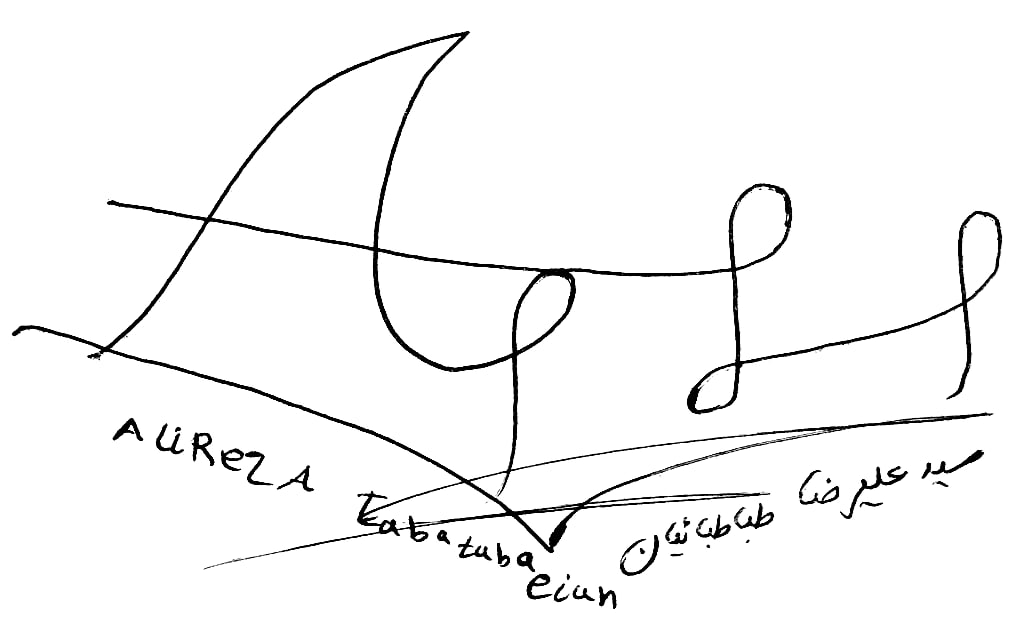
\includegraphics[scale=0.2]{Signature}
\end{wrapfigure}

\vspace{-1cm}
{\centerline {\bf{\fname\lname}}}
\vspace*{.2cm}
{\centerline{امضا}}
%%%%%%%%%%%%%%%%%%%%%%%%%%%%%%%%%
% چنانچه مایل به چاپ صفحات «تقدیم»، «نیایش» و «سپاس‌گزاری» در خروجی نیستید، خط‌های زیر را با گذاشتن ٪  در ابتدای آنها غیرفعال کنید.
% پایان‌نامه خود را تقدیم کنید
% نیایش خود را در فایل زیر بنویسید.
\begin{acknowledgementpage}

\vspace{1.5cm}

{\nastaliq
{
 نويسنده پايان‌نامه، درصورت تمايل ميتواند برای سپاسگزاری پايان‌نامه خود را به شخص يا اشخاص و يا ارگان خاصی تقدیم نماید.
}}\end{acknowledgementpage}
\newpage
% سپاسگزاری را در فایل زیر بنویسید.
%%%%%%%%%%%%%%%%%%%%%%%%%%%%%%%%%%%%
\newpage\thispagestyle{empty}
% سپاس‌گزاری
{\nastaliq
سپاس‌گزاری
}
\\[2cm]

 نويسنده پايان‌نامه می‌تواند مراتب امتنان خود را نسبت به استاد راهنما و استاد مشاور و یا ديگر افرادي كه طي انجام پايان‌نامه به نحوي او را یاری و یا با او همكاری نموده‌اند ابراز دارد.














% با استفاده از دستور زیر، امضای شما، به طور خودکار، درج می‌شود.
\signature








%%%%%%%%%%%%%%%%%%%%%%%%%%%%%%%%%%%%%%%%%
%%%%%%%%%%%%%%%%%%%%%%%%%%%%%%%%%کدهای زیر را تغییر ندهید.
\newpage\clearpage

\pagestyle{style2}

\vspace*{-1cm}
\section*{\centering چکیده}
%\addcontentsline{toc}{chapter}{چکیده}
\vspace*{.5cm}
\ffa-abstract
\vspace*{2cm}


{\noindent\large\textbf{واژه‌های کلیدی:}}\par
\vspace*{.5cm}
\fkeywords
% دستور زیر برای شماره گذاری صفحات قبل از فصل اول با حروف ابجد است.
\pagenumbering{alph}
%-----------------------------------------------------------------------------
% فایل زیر دستورات مربوط به نمایش صفحات فهرست مطالب- فهرست اشکال و جداول است.
%{\pagestyle{style2}
%\tableofcontents}\newpage
%
%\listoffigures
\cleardoublepage
\pagestyle{style6}
\tableofcontents
\pagestyle{style6}
\cleardoublepage
%اگر لیست تصاویر و لیست جداول ندارید ، کدهای زیر را با گذاشتن % در ابتدای آنها، غیرفعال کنید.
\BeginNoToc
%============
\addtocontents{lof}{\lofheading}% add heading to the first page in LoF
\pagestyle{style5}
\listoffigures
\thispagestyle{style5}
\cleardoublepage
%============
\addtocontents{lot}{\lotheading}% add heading to the first page in LoT
\thispagestyle{style4}
\listoftables
\thispagestyle{style4}
%============
%\cleardoublepage
%
\cleardoublepage
\setcounter{savepage}{\arabic{page}}
\mainmatter
\addtocontents{toc}{\tocheading}% add heading to the first page in ToC, after frontmatter entries
\EndNoToc
% در صورت تمایل می‌توانید با فعال کردن دستور بالا، لیست تصاویر را به  پایان‌نامه خود اضافه کنید.
%-------------------------------------------------------------------------symbols(فهرست نمادها)
% وجود لیست نمادها الزامیست.(لطفاً نمادهای خود را جایگذین نمادهای پیش‌فرض کنید.)
%%%%%%%%%%%%%

{\centering\LARGE\textbf{فهرست نمادها}\par}%

\pagenumbering{alph}
\setcounter{page}{\thesavepage}
%\setcounter{page}{6}
\vspace*{1cm}

\pagestyle{style3}
%\thispagestyle{empty}
%\addcontentsline{toc}{chapter}{فهرست نمادها}
\symb{\text{ نماد}}{مفهوم}
\\
%مقادیر بالا را تغییر ندهید
%%%%%%%%%%%%%%%%%%%%%%%%%%%%%%%%%%%%%%%%%%%%%%%%%%%%%%%%%
\symb{N}{تعداد المان‌های آنتن}
\symb{M_1}{تعداد المان‌های سطح هوشمند اول}
\symb{M_2}{تعداد المان‌های سطح هوشمند دوم}
\symb{w_1}{وزن نرخ کاربر اول}
\symb{w_2}{وزن نرخ کاربر دوم}
\symb{P_t}{ماکسیمم توان دو کاربر}
\symb{\sigma}{انحراف از معیار نویز}
\symb{\sigma^2}{توان نویز}
\symb{n}{ضریف افت توان}
\symb{D}{کانال بین دو سطح هوشمند}
\symb{G}{کانال بین آنتن و سطوح هوشمند}
\symb{h}{کانال منتهی به کاربر}
\symb{\gamma}{نرخ دریافتی کاربر}
\symb{s}{سمبل دریافتی کاربر}
\symb{y}{کل سیگنال دریافتی کاربر بهمراه نویز}
\symb{\phi}{ماتریس قطری ضرایب تغییر فاز سطوح هوشمند}
\symb{\alpha}{متغیر اختیاری}
\symb{\beta}{متغیر اختیاری}
\symb{\lambda}{متغیر اختیاری کنترل توان}
\symb{\epsilon}{متغیر اختیاری}
\symb{\theta}{بردار ضرایب تغییر فاز سطوح هوشمند}
\symb{j}{نماد عدد مختلط}
\symb{C^{m * n}}{ماتریس مختلط با \lr{m} سطر و \lr{n} ستون}
\symb{Re(.)}{مقدار حقیقی یک عدد}
\symb{Im(.)}{مقدار مختلط یک عدد}

%%%%%%%%%%%%%%%%%%%%%%%%%%%%%%%%%%%%%%%

\thispagestyle{style3}
\newpage
%\pagestyle{style1}
%%%%%%%%%%%%%%%%%%%%%%%%%%%%%%%%%%%%


\pagenumbering{arabic}
\pagestyle{style1}
%--------------------------------------------------------------------------chapters(فصل ها)
\chapter{علم مخابرات}
در این فصل ابتدا علم مخابرات را تعریف و اصول اساسی آن را بررسی میکنیم. سپس به کاربردها و گستره این علم میپردازیم. در ادامه با بیان تاریخچه آن، درکی نسبی از این علم پیدا میکنیم. سپس بر بخش خاصی از مخابرات به‌نام مخابرات بیسیم یا مخابرات سیار و سپس مخابرات سلولی متمرکز میشویم. در نهایت نیز انواع فرستنده-گیرنده را از حیث تعداد آنتن بررسی کرده و مفهوم کلی سطوح بازتاب‌دهنده هوشمند و کاربردهای آن را مورد بررسی قرار میدهیم.
\newpage
%%%%%%%%%%%%%%%%%%%%%%%%%%%%%%%%%%%%%%%%%%%
\section{مقدمه‌ای بر علم مخابرات}
علم مخابرات یک رشته مهم و چندگانه‌ای است که به مطالعه انتقال، تبادل و تفسیر اطلاعات بین افراد، سیستم‌ها و دستگاه‌ها می‌پردازد. این علم به دنبال بهبود کارایی و امنیت انتقال اطلاعات در فرآیندهای مختلف می‌باشد. مخابرات تأثیر بسزایی بر توسعه اجتماعی، اقتصادی و فناوری دارد و در زمینه‌های مختلفی نظیر تلفن، اینترنت، تلویزیون و ارتباطات نظامی به کار می‌رود.

\subsection{
	اصول اساسی مخابرات
}
\begin{enumerate}
	\item \textbf{
		انتقال اطلاعات:
	}
	 عملیات انتقال داده‌ها و اطلاعات از یک مکان به مکان دیگر از اصول اساسی مخابرات است. این انتقال می‌تواند به صورت سیمی (مانند کابل‌ها) یا بی‌سیم (از طریق امواج رادیویی یا مایکروویو) انجام شود.
	
	\item \textbf{مدولاسیون و دمدولاسیون:} برای انتقال اطلاعات، آن‌ها به سیگنال‌هایی تبدیل می‌شوند که به راحتی قابل انتقال باشند. این فرآیند به نام مدولاسیون شناخته می‌شود. در مقابل، دمدولاسیون فرآیند بازیابی اطلاعات از سیگنال‌های مدوله شده را شامل می‌شود.
	
	\item \textbf{کدگذاری و کدگشایی:} برای افزایش امنیت و کاهش تداخلات، اطلاعات ممکن است با استفاده از روش‌های کدگذاری به یک فرمت خاص تبدیل شوند. کدگشایی نیز فرآیند بازگرداندن اطلاعات به فرمت اصلی را توصیف می‌کند.
\end{enumerate}

\section{کاربردها و گستره علم مخابرات}
\subsection{کاربردهای اصلی مخابرات}
\begin{enumerate}
	\item \textbf{تلفنی و تصویری:} انتقال صدا و تصاویر در عصر حاضر از طریق تلفن و ویدئوکنفرانس از کاربردهای اصلی مخابرات به شمار می‌آید.
	
	\item \textbf{شبکه‌های کامپیوتری:} اینترنت و شبکه‌های دیگر از راه‌های ارتباطی بر اساس اصول مخابراتی هستند که به ما امکان ارسال و دریافت اطلاعات را از سراسر جهان می‌دهند.
	
	\item \textbf{تلویزیون و رادیو:} انتقال برنامه‌های تلویزیونی و رادیویی به تلویزیون‌ها و رادیوها نیز از طریق اصول مخابراتی انجام می‌شود.
	
	\item \textbf{تله‌مدیسین و تله‌پزشکی:} از مخابرات برای انتقال اطلاعات پزشکی و تصاویر پزشکی به منظور تشخیص بیماری‌ها و مشاوره‌ی پزشکی از راه دور استفاده می‌شود.
	
	\item \textbf{ارتباطات فضایی:} در ماموریت‌های فضایی و ارتباطات با ماهواره‌ها، اصول مخابراتی برای ارسال و دریافت اطلاعات به‌کار می‌روند.
	
	\item \textbf{شبکه‌های اجتماعی:} ارتباطات اجتماعی آنلاین از طریق شبکه‌های اجتماعی نیز از تکنیک‌های مخابراتی برای انتقال اطلاعات استفاده می‌کنند.
\end{enumerate}

\subsection{گستره علم مخابرات}
علم مخابرات به وسیع‌ترین معانی به سایر حوزه‌های علمی نیز ارتباط دارد. به عنوان مثال:
\begin{itemize}
	\item \textbf{مخابرات نظامی:} در ارتباطات نظامی، امنیت، ردیابی، جاسوسی و انتقال داده‌ها در شرایط خاص مورد بررسی قرار می‌گیرد.
	
	\item \textbf{پزشکی:} از مخابرات در تله‌مدیسین، انتقال تصاویر پزشکی و اطلاعات بیماری‌ها برای تشخیص از راه دور استفاده می‌شود.
	
	\item \textbf{حمل و نقل:} ارتباطات در خودروها، قطارها و هواپیماها جهت بهبود امنیت و کارایی حمل و نقل مورد استفاده قرار می‌گیرد.
	
	\item \textbf{تکنولوژی اطلاعات و ارتباطات (\lr{ICT}):} علم مخابرات به‌عنوان پایه‌ای از علوم مرتبط با \lr{ICT}، به توسعه ابزارها، سیستم‌ها و نرم‌افزارهای ارتباطی کمک می‌کند.
	
	\item \textbf{امنیت اطلاعات:} در دنیای امروز، امنیت اطلاعات و محرمانگی داده‌ها نقش بسزایی دارد که از اصول مخابراتی برای رمزنگاری و حفاظت در برابر نفوذ استفاده می‌شود.
	
	\item \textbf{شبکه‌های هوش مصنوعی:} انتقال داده‌ها و اطلاعات در شبکه‌های هوش مصنوعی و اینترنت اشیاء نیز از اصول مخابراتی بهره می‌برد.
\end{itemize}

علم مخابرات به دلیل تأثیرات وسیع‌تری که بر ابزارها، فرآیندها و جوامع دارد، به یکی از پایه‌های اصلی توسعه فناوری و ارتباطات در جوامع مدرن تبدیل شده است. این علم به دنبال بهبود ارتباطات بین انسان‌ها و دستگاه‌ها در سراسر جهان است و در عصر اطلاعات، نقش بسزایی دارد.
%%%%%%%%%%%%%%%%%%%%%%%%%%%%%%%%%%%%%%%%%%%
\section{آغاز و پیشینه تاریخی علم مخابرات}

در طول تاریخ، انسان‌ها همواره تلاش کرده‌اند تا ارتباطات خود را بهبود بخشند. از ارسال پیغام‌های ساده با کمک آتش یا دیگر علائم تا به اختراع وسایل پیام‌رسان پیشرفته، مراحل مختلفی در تاریخچه مخابرات وجود دارد.

\subsection{سازوکارهای اولیه}
در دوران‌های اولیه تاریخ، ارتباطات انسان‌ها از طریق نمادها، علائم و صداها انجام می‌شد. انسان‌ها از طریق آتش و دود، نشانه‌های راهبردی می‌ساختند که از دور قابل مشاهده بودند. همچنین، استفاده از پیغام‌های صوتی با استفاده از زنگ‌ها و دستگاه‌های ساده دیگر از مکانیسم‌های اولیه مخابرات بود.

\subsection{استفاده از حیوانات و افراد}
با گذر زمان، انسان‌ها از حیوانات و افراد برای انتقال پیغام‌ها و اطلاعات به فاصله‌های بیشتر استفاده کردند. از پیغام‌رسانی با استفاده از کوفی‌ها و مسیریابی پیاده‌روی‌ها تا ایجاد سیستم‌هایی برای انتقال پیام‌ها با استفاده از اسب‌ها، مثال‌هایی از این دوران‌ها هستند.

\subsection{اختراع رادیو}
با پیشرفت فناوری در قرن 19، اختراع رادیو توسط علمایی چون گوگلیلمو مارکونی و نیکولا تسلا انقلابی در زمینه مخابرات ایجاد کرد. رادیو به انسان‌ها امکان ارسال و دریافت امواج الکترومغناطیسی را به صورت بی‌سیم فراهم کرد و ارتباطات بی‌سیم را آغاز کرد.
%%%%%%%%%%%%%%%%%%%%%%%%%%%%%%%%%%%%%%%%%%%
\section{تکنولوژی مخابرات در قرن بیست و یکم}
در قرن بیست و یکم، پیشرفت‌های فراوانی در زمینه علم مخابرات رخ داد. با ظهور کامپیوترها و توسعه اینترنت، ارتباطات به طور جهانی و پیچیده‌تری انجام می‌شود. فناوری‌های بی‌سیم مانند موبایل، وای‌فای، بلوتوث و ماهواره‌ها ارتباطات را به سطح جدیدی رسانده‌اند.

\subsection{انقلاب دیجیتالی و اینترنت}
در دهه‌های اخیر، انقلاب دیجیتالی و ظهور اینترنت تغییرات اساسی در مخابرات ایجاد کرده‌اند. اینترنت به عنوان یک شبکه جهانی، میلیاردها دستگاه را به یکدیگر متصل کرده و به اشتراک گذاری اطلاعات، ارتباطات اجتماعی و تجارت را تغییر داده است.

\subsection{شبکه‌های اجتماعی و ارتباطات اجتماعی آنلاین}
با ظهور شبکه‌های اجتماعی مانند فیسبوک، توییتر، اینستاگرام و لینکدین، ارتباطات اجتماعی به صورت آنلاین و از راه دور انجام می‌شود. این شبکه‌ها نه تنها به اشتراک گذاری تجربیات و اطلاعات، بلکه در پیدا کردن کار، تبلیغات و تأثیرگذاری نیز نقش دارند.

\subsection{مخابرات \lr{5G} و پیشرفت‌های آینده}
تکنولوژی مخابرات همچنان در حال پیشرفت است. به عنوان مثال، فناوری \lr{5G} با امکانات بالاتری در سرعت انتقال داده، کاهش تأخیر و افزایش توانایی اتصال بهتر، در حال توسعه است و قرار است تاثیرات چشمگیری بر ارتباطات و صنایع داشته باشد.
%%%%%%%%%%%%%%%%%%%%%%%%%%%%%%%%%%%%%%%%%%%
\section{
	مخابرات سیار یا مخابرات بیسیم
}

\subsection{
	تعریف
}
مخابرات سیار یا مخابرات بیسیم به انتقال اطلاعات و ارتباطات بین دستگاه‌ها از طریق امواج رادیویی یا وسایل بی‌سیم مشغول است. این فناوری به ما این امکان را می‌دهد که در هر مکانی و در هر زمانی ارتباط داشته باشیم، بدون نیاز به سیم‌کشی یا اتصال فیزیکی مستقیم.

\subsection{تاریخچه مخابرات بیسیم}
مخابرات بیسیم از زمان اختراع رادیو تا به امروز تغییرات بزرگی را تجربه کرده است. اختراع تلگراف بیسیم توسط مارکونی در اواخر قرن نوزدهم توسط وایرلس تلگراف راه‌اندازی شد. پس از آن، با اختراع رادیو و سایر فناوری‌های بی‌سیم، مخابرات بیسیم به شکلی کاملاً جدید تبدیل شد.

\subsection{انواع مخابرات بیسیم}
مخابرات بیسیم به انواع مختلفی تقسیم می‌شود. از جمله انواع مخابرات بیسیم می‌توان به مخابرات سلولی، وای‌فای، بلوتوث، نسل‌های مختلف تلفن همراه مانند \lr{3G}, \lr{4G}
 و \lr{5G}
 و ارتباطات ماهواره‌ای اشاره کرد.

\subsection{کاربردهای مخابرات بیسیم}
مخابرات بیسیم در زندگی روزمره ما نقش بزرگی ایفا می‌کند. از تماس‌های تلفنی و پیامک‌ها تا استفاده از اینترنت بی‌سیم، تلویزیون‌های هوشمند، دستگاه‌های هوشمند، سامانه‌های ردیابی موقعیت جغرافیایی، سیستم‌های اطلاع‌رسانی اضطراری و بسیاری از فناوری‌های دیگر، مخابرات بیسیم به‌طور گسترده در حیات ما حضور دارد.
%%%%%%%%%%%%%%%%%%%%%%%%%%%%%%%%%%%%%%%%%%%
\section{
	مخابرات سلولی
}

\subsection{تعریف}
مخابرات سلولی، یا شبکه‌های تلفن همراه، سیستم‌های ارتباطی بی‌سیم هستند که از امواج رادیویی برای انتقال صدا، داده و اطلاعات استفاده می‌کنند. این سیستم‌ها به دستگاه‌های تلفن همراه اجازه می‌دهند تا به تبادل اطلاعات با یکدیگر و به شبکه ارتباطی متصل شوند.

\subsection{تقسیمات شبکه‌های سلولی}
شبکه‌های تلفن همراه به چندین منطقه تقسیم می‌شوند که به این مناطق سلول‌ گفته می‌شود. هر سلول یک محدوده جغرافیایی را پوشش می‌دهد و دارای یک تجهیزات ارتباطی مرکزی است که به عنوان ترانس‌هدایت‌کننده مرکزی (\lr{BTS}) شناخته می‌شود.

\subsection{تکنولوژی‌های نسل‌های مختلف تلفن همراه}
شبکه‌های تلفن همراه در طول زمان به نسل‌های مختلفی تقسیم می‌شوند که به توانایی‌های خاص خود معروف هستند. از نسل اول تا نسل پنجم، هر نسل به سرعت انتقال داده، پهنای باند، قابلیت‌های صوتی و تصویری و کاربردهای دیگر ارتباطات بی‌سیم تاثیر می‌گذارد.

\subsection{تغییرات اجتماعی و اقتصادی از طریق مخابرات سلولی}
مخابرات سلولی تغییرات عمده‌ای در جوامع و اقتصادها به وجود آورده است. از تجارت الکترونیک و کسب‌وکارهای آنلاین گرفته تا ارتباطات اجتماعی و تغییرات در رفتارهای انسانی، این تکنولوژی اثرات چشمگیری را در سطح جامعه داشته است.
%%%%%%%%%%%%%%%%%%%%%%%%%%%%%%%%%%%%%%%%%%%
\section{انواع فرستنده-گیرنده از نظر تعداد آنتن}

\subsection{
	ارتباط \lr{SISO} : تک ورودی - تک خروجی
}

ارتباط \lr{SISO}، مخفف \lr{Single-Input Single-Output}، یک سیستم ارتباطی بی‌سیم ابتدایی است که در آن یک فرستنده تنها از یک آنتن برای ارسال سیگنال به یک گیرنده استفاده می‌کند. در این تنظیم، یک آنتن در فرستنده و یک آنتن در گیرنده وجود دارد. ارتباط در جهت یکطرفه است، به این معنی که فرستنده اطلاعات را ارسال کرده، و گیرنده آن را دریافت می‌کند.

سیستم‌های تک ورودی - تک خروجی در کاربردهای مختلفی از جمله پخش رادیویی سنتی، دستگاه‌های واکی‌تاکی و بسیاری از سیستم‌های ارتباطی بی‌سیم اولیه استفاده می‌شوند. با وجود سادگی، سیستم‌های تک ورودی - تک خروجی محدودیت‌هایی در زمینه نرخ داده، محدوده پوشش و قابلیت اطمینان دارند. تداخل، خنثی شدن و نویز ممکن است بر کیفیت سیگنال دریافتی نیز تأثیر بگذارد.

\subsection{
	ارتباط \lr{MISO} : چند ورودی - تک خروجی
}

ارتباط \lr{MISO}، مخفف \lr{Multiple-Input Single-Output}، در شرایطی به کار می‌رود که یک گیرنده تنها سیگنال‌ها را از چند فرستنده متفاوت که هرکدام دارای آنتن خود هستند، دریافت می‌کند. این تنظیم برای بهبود کیفیت سیگنال، پوشش و نرخ داده مورد استفاده قرار می‌گیرد. چندین فرستنده می‌توانند با همکاری به تقویت قدرت سیگنال دریافتی و کاهش تأثیر خنثی شدن و خنثی شدگی کمک کنند.

سیستم‌های \lr{MISO} اغلب در شبکه‌های سلولی به کار می‌روند، جایی که چندین ایستگاه پایه سیگنال‌ها را به یک دستگاه تلفن همراه ارسال می‌کنند. دستگاه تلفن همراه از طریق ترکیب سیگنال‌ها از آنتن‌های مختلف به کیفیت سیگنال دریافتی بهتری دست می‌یابد. این تنظیم به حل مشکلاتی مانند خنثی شدن چندمسیره و اثر سایه ای کمک می‌کند و باعث بهبود کیفیت ارتباط می‌شود.

\subsection{
		ارتباط \lr{SIMO} : تک ورودی - چند خروجی
}

ارتباط \lr{SIMO}، مخفف \lr{Single-Input Multiple-Output}، به سیستمی اشاره دارد که یک فرستنده تنها سیگنال را به چندین گیرنده ارسال می‌کند، هر کدام دارای آنتن خود هستند. این تنظیم امکان دریافت تنوعی را فراهم می‌کند، به طوری که گیرنده‌های چندگانه سیگنال را از مسیرهای مختلف دریافت می‌کنند. این کار باعث مقابله با محوشوندگی و بهبود قابلیت اطمینان ارتباط می‌شود.

سیستم‌های \lr{SIMO} در مواقعی مورد استفاده قرار می‌گیرند که ارتباط قابل اعتماد بسیار مهم است، مانند ارتباطات بی‌سیم در محیط‌های چالشی یا پوشش دهی داخلی. با استفاده از چندین آنتن در سمت گیرنده، تأثیرات انتشار چندمسیره و محوشوندگی می‌تواند کاهش یابد و از این رو کیفیت ارتباط بهبود می‌یابد.

\subsection{
	ارتباط \lr{MIMO} : چند ورودی - چند خروجی
}

ارتباط \lr{MIMO}، مخفف \lr{Multiple-Input Multiple-Output}، یک سیستم پیشرفته ارتباطی بی‌سیم است که همزمان از چندین آنتن در فرستنده و گیرنده استفاده می‌کند. تکنولوژی \lr{MIMO} از تنوع فضایی و انتشار چندمسیره برای دستیابی به نرخ داده، پوشش و اطمینان بیشتر استفاده می‌کند. چندین جریان داده می‌توانند به صورت همزمان روی همان فرکانس ارسال شوند که باعث افزایش ظرفیت سیستم می‌شود.

سیستم‌های \lr{MIMO} به عنوان یک تکنولوژی بنیادی در استانداردهای ارتباطی بی‌سیم مدرن، از جمله \lr{Wi-Fi} و شبکه‌های سلولی (مانند \lr{4G} و \lr{5G}) به کار می‌روند. با استفاده از چندین آنتن، سیستم‌های \lr{MIMO} می‌توانند از تنوع فضایی برای بهبود کیفیت سیگنال، مهار تداخل و دستیابی به نرخ داده بالاتر استفاده کنند.
%%%%%%%%%%%%%%%%%%%%%%%%%%%%%%%%%%%%%%%%%%%
\section{
	سطوح بازتاب دهنده هوشمند (\lr{IRS})
}

\subsection{
	مفهوم کلی
}

سطوح بازتاب دهنده هوشمند همچنین با نام‌های سطوح بازتاب‌کننده قابل تنظیم یا سطوح بازتاب دهنده هوشیار، فناوری پیشرفته‌ای در ارتباطات بی‌سیم و پردازش سیگنال هستند. این ایده شامل استفاده از سطوحی با عناصر غیرفعال(\lr{passive}) نمایش داده می‌شود که برای کنترل و مدیریت امواج الکترومغناطیسی به کار می‌روند. با تغییر بازتاب و پراکندگی سیگنال‌ها، سطور بازتاب‌دهنده هوشمند می‌تواند کیفیت سیگنال‌ها را افزایش داده، پوشش را افزایش داده و عملکرد کلی سیستم‌های ارتباطی بی‌سیم را بهبود بخشد. در ادامه، مروری اجمالی از این سطوح و کاربردهای آن آورده شده است:

\subsection{
	اصول کار
}

\lr{IRS} شامل یک سطح با عناصر غیرفعال کوچک مانند آنتن‌ها، سوئیچ‌ها یا مواد قابل تنظیم می‌شود. این عناصر می‌توانند فاز و مقدار موج‌های الکترومغناطیسی ورودی را تغییر دهند. با تنظیم دقیق فاز و مقدار، \lr{IRS} می‌تواند سیگنال‌ها را در جهات مورد نظر بازتاب کند تا تداخل سازنده ایجاد کرده و قدرت سیگنال در گیرنده را بهبود دهد.

\subsection{کاربردهای سطوح هوشمند}

- \textbf{
	افزایش کیفیت ارتباط بی‌سیم:
}
 یکی از کاربردهای اصلی سطوح هوشمند، بهبود کیفیت و پوشش سیستم‌های ارتباطی بی‌سیم است. با تغییر سیگنال‌های بازتابی، می‌توان اثر تداخل‌های چندمسیره را کاهش داده، نسبت سیگنال به نویز را بهبود داده و پوشش را به مناطقی با سیگنال ضعیف ترتیب دهد.

- \textbf{
	پوشش داخلی و نفوذ:
}
 \lr{IRS} می‌تواند در محیط‌های داخلی برای رفع مشکلات نفوذ سیگنال به دلیل دیوارها، مبلمان و موانع دیگر استفاده شود. این فناوری می‌تواند نفوذ سیگنال و پوشش را بهبود داده و ارتباطات داخلی را قابل اعتماد‌تر کند.

- \textbf{
	\lr{5G} و به بعد:
} \lr{IRS}
 در شبکه‌های \lr{5G} و سیستم‌های ارتباطی آینده توانمندی‌های بسیاری دارد. این وسیله می‌تواند به زیرساخت‌های سلولی موجود اضافه شود تا نرخ داده را بهبود داده، تاخیر را کاهش داده و ظرفیت شبکه را افزایش دهد.

- \textbf{کارآیی انرژی:} \lr{IRS} نیز می‌تواند به بهبود کیفیت سیگنال‌های دریافتی کمک کند و به دستگاه‌ها اجازه دهد با توان کمتر عمل کنند که این منجر به صرفه‌جویی در مصرف انرژی می‌شود.

- \textbf{ارتباطات امن:} با کنترل جهت سیگنال و کاهش نفوذ سیگنال به مناطق غیر مجاز می‌تواند به افزایش امنیت ارتباط کمک کند.

- \textbf{اینترنت اشیا (\lr{IoT}):} در سناریوهای اینترنت اشیا که تعداد زیادی دستگاه با یکدیگر ارتباط دارند، سطوح هوشمند می‌تواند به بهبود کارآیی و قابلیت اعتماد شبکه کمک کند.

- \textbf{ترکیب \lr{Massive MIMO}:} \lr{IRS} می‌تواند با سیستم‌های \lr{MIMO} بزرگ ترکیب شود تا عملکرد آن‌ها را بهبود دهد و سیستم ترکیبی با اجزای فعال و غیرفعال ایجاد کند.

- \textbf{شکل‌دهی به شعاع و جهت:} \lr{IRS} با شکل‌دهی به شعاع و جهت دینامیک اجازه می‌دهد تا با تطابق به شرایط مختلف ارتباطات پیش بروید.

\subsection{چالش‌ها و چشم‌اندازهای آینده}

با وجود مزایای فراوان، مواردی مانند پیاده‌سازی عملی، همگام‌سازی و تخمین کانال در مورد \lr{IRS} چالش‌هایی وجود دارد. با این حال، تحقیقات و توسعه‌های جاری به منظور غلبه بر این موانع و بهره‌برداری کامل از تکنولوژی سطوح هوشمند در حال انجام است.

\subsection{نتیجه‌گیری}

سطوح بازتاب دهنده هوشمند نشان‌دهنده یک فناوری تحول‌آفرین در ارتباطات بی‌سیم هستند. توانایی این فناوری در تغییر موج‌های الکترومغناطیسی، امکانات جدیدی را برای بهبود کیفیت سیگنال‌ها، پوشش و ظرفیت ارتباطات ارائه می‌دهد. در حالی که تحقیقات و نوآوری‌ها ادامه دارند، انتظار می‌رود که این سطوح نقش اساسی را در تدوین آینده سیستم‌های ارتباطات بی‌سیم ایفا کند.

\newpage
‌
\chapter{طریقه‌ی مرجع نویسی و واژه‌نامه‌}
\section{طریقه‌ی مرجع نویسی}
برای نوشتن مراجع پایان نامه، برای راحتی کار به صورت زیر عمل می‌کنیم:
\subsection{بارگیری مراجع}
در ابتدا مراجع را باید از سایت‌های معتبر بارگیری کنیم، مثلا برای ارجاع دادن به مقاله‌ی
\lr{A classification of some Finsler connections and their applications}
ابتدا به سایت
\href{scholar.google.com}{گوگل اسکولار} 
رفته و این مقاله را جستجو می‌کنیم. پس از پیدا کردن این مقاله، مانند شکل زیر، در زیر نام و چکیده‌ی مقاله، $5$ گزینه وجود دارد که عبارتند از:\\

\begin{enumerate}
\item \lr{ Cited by}

\item \lr{ Related articles}

\item \lr{ All 6 versions}

\item \lr{ Cite}

\item \lr{ Save}
\end{enumerate}
\begin{figure}[!h]
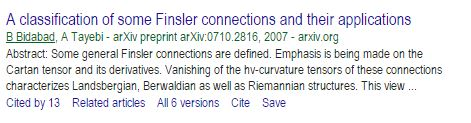
\includegraphics[height=3cm]{bidabad}
\caption{نمونه یک مقاله در گوگل اسکولار}
\end{figure}
در اینجا ما به گزینه‌ی چهارم یعنی
\lr{ Cite}
احتیاج داریم. بر روی آن کلیک کرده و پنجره‌ای مانند
\cref{fig.2}
باز می‌شود که دارای $4$ گزینه‌ی زیر است:
\begin{enumerate}
\item \lr{BibTeX}

\item \lr{EndNote}

\item \lr{RefMan}

\item \lr{RefWorks}
\end{enumerate}
\begin{figure}
\centering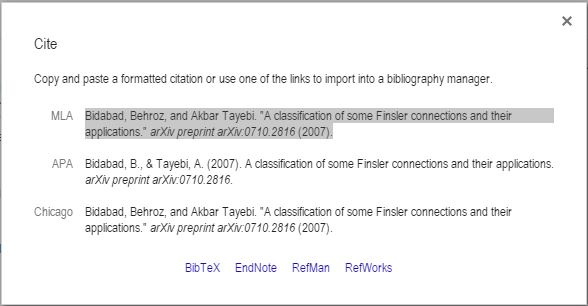
\includegraphics[scale=.6]{bibref}
\caption{پنجره‌ی باز شده در گوگل اسکولار}\label{fig.2}
\end{figure}
روی گزینه‌ی اول، یعنی
\verb;BibTeX;
کلیک کرده و همه‌ی نوشته‌های پنجره‌ی باز شده را مانند زیر، کپی کرده و در فایل
\verb;references.bib;
موجود در فایل
\verb;AUTthesis;
پیست می‌کنیم. سپس کلیدهای
\verb;Ctrl+s;
را می‌زنیم تا فایل ذخیره شود.\\
\begin{latin}
	\normalsize
\begin{verbatim}
@ article{bidabad2007classification,
title={A classification of some Finsler connections and their applications},
author={Bidabad, Behroz and Tayebi, Akbar},
journal={arXiv preprint arXiv:0710.2816},
year={2007}
}
\end{verbatim}
\end{latin}
\subsection{روش ارجاع در متن}
برای ارجاع دادن به مقاله‌ی بالا، باید در جایی که می‌خواهید ارجاع دهید، دستور زیر را تایپ کنید:
\begin{latin}
\lr{$\backslash$cite\{bidabad2007classification\}}
\end{latin}
همانطور که مشاهده می‌کنید از کلمه‌ای که در سطر اول ادرس مقاله آمده (یعنی کلمه‌ی پس از
\lr{@article$\lbrace$})
استفاده کرده‌ایم. پس از دستور فوق، به صورت \cite{bidabad2007classification} و \cite{aa} مرجع خواهد خورد. توجه شود که در صورتی مراجع چاپ خواهند شد که در متن به انها ارجاع داده شده باشد. همچنین برای ارجاع چندتایی از دستور 
\lr{$\backslash$cite\{name1, name2,...\}}
استفاده کنید که به‌صورت \cite{najafi2008finsler, zakeri, najafi} ارجاع خواهند خورد.
\subsection{روش اجرای برنامه}
ابتدا فایل
\verb;AUT_thesis.tex;
را باز کرده و آن را دو بار اجرا کنید. سپس حالت اجرا را از 
\verb;Build Quick;
به حالت
\verb;Bibtex;
تغییر داده و دوباره برنامه را اجرا کنید. دو بار دیگر برنامه را در حالت 
\verb;Build Quick;
اجرا کرده و نتیجه را مشاهده کنید. در این روش تمامی مراجع بر اساس اینکه کدام یک در متن زودتر به آن ارجع داده شده لیست خواهند شد.
\subsection{مراجع فارسی}
برای نوشتن مراجع فارسی باید به صورت دستی، در همان فایل قبلی به صورت زیر عمل می‌کنیم:
\begin{LTR}
\noindent\verb;@article{manifold,;\\
\verb;title={;منیفلد هندسه\verb;},;\\
\verb;author={;بیدآباد دکتربهروز \verb;},;\\
\verb;journal{; امیرکبیر صنعتی دانشگاه\verb;},;\\
\verb;year={1389},;\\
\verb;LANGUAGE={Persian};\\
\verb;};
\end{LTR}
همانطور که مشاهده می‌کنید تنها تفاوت آن با حالت مراجع انگلیسی، سطر آخر آن می‌باشد که زبان را مشخص می‌کند که حتماً باید نوشته شود.
\section{راهنمای واژه‌نامه}

به دلیل پیچیدگی واژه‌نامه‌های موجود در سایت پارسی لاتک، از روش زیر برای نوشتن واژه‌نامه استفاده کنید:

ابتدا با استفاده از اکسل، واژه های خود را یک‌بار براساس حروف الفبای فرسی و بار دیگر انگلیسی مرتب کنید. سپس واژه ها را در فایل \lr{dicen2fa} و \lr{dicfa2en} قرار دهید.

\section{ساخت نمایه}\label{Namaye}
\subsection{ساخت نمایه}
 \begin{enumerate}

\item
کلمات مورد نظر خود مثلا \lr{word} با دستور \verb|\index{word}| ایندکس کنید.
\item
نحوه‌ی اجرای \lr{Make Index}   در ویرایشگرهای \lr{TeX Maker} و \lr{TeX Works}:
\begin{itemize}
\item  تک‌میکر: از منوی \lr{Tools} گزینه‌ی \lr{Xindy Make Index} را کلیک کنید یا از دکمه‌‌های میانبر \lr{Ctrl+Alt+I} استفاده کنید.

\item  تک‌ورکز: ابتدا باید مثل عکس زیر تنظیم  و سپس گزینه‌ی \lr{Xindy Make Index}  انتخاب و روی دکمه‌ی سبز رنگ کلیک کنید یا از دکمه‌های  \lr{Ctrl+T} استفاده کنید.

\begin{figure}[!h]
\centerline{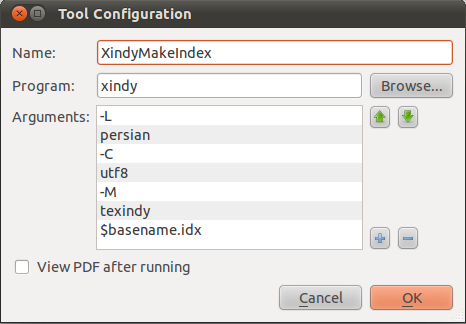
\includegraphics[width=.5\textwidth]{Xindy_Make_Index.png}}
\caption{تنظیمات مربوط به تک‌ورکز}
\end{figure}

\end{itemize}
 \end{enumerate}
 
 \index{کتاب}
\index{پارسی‌لاتک}
\index{بی‌دی}
\index{سوال}
\index{عنصر}
\index{گزینه}
\index{ژاکت}
\index{مرکز دانلود}
\index{اجرا}
\index{تک‌لایو}
\index{ثالث}
\index{جهان}
\index{چهار}
\index{حمایت}
\index{خواهش}
\index{دنیا}
\index{زی‌پرشین}
\index{ریحان}
\index{شیرین}
\index{صمیمی}
\index{ضمیر}
\index{طبیب}
\chapter{کارهای پیشین و سناریوی مسئله}
در این فصل ابتدا انواع مسائل مطرح شده در زمینه سطوح بازتاب‌کننده هوشمند را بررسی میکنیم و سپس مسائلی که تا حدودی با سناریوی ما شبیه است یا به درک بهتر این سناریو کمک میکند را بصورت سطحی بررسی میکنیم. در نهایت نیز سناریوی مورد تحلیل را شرح داده و تفاوت این سناریو را با سایر سناریوها بررسی میکنیم.
%%%%%%%%%%%%%%%%%%%%%%%%%%%%%%%%%%%%%%%%%%%
\section{
	انواع مسائل مطرح‌شده در زمینه سطوح بازتاب‌کننده\\ هوشمند
 }

در زمینه سطوح بازتاب کننده هوشمند، مسائل مختلفی مطرح است. یکی از دسته‌بندی‌های کلی مسائل مطرح شده در این زمینه، به شرح زیر است:

\newpage

\subsection{مسائل میدانی:}
\begin{itemize}
	\item 
	طراحی سطوح هوشمند: یکی از چالش‌هایی که همواره دانشمندان و محققان در حال دست و پنجه نرم کردن با آن هستند، طراحی سطوح هوشمند در تعداد بالا و با هزینه پایین میباشد. البته سطوح هوشمند تا کنون در ابعاد کوچک و بصورت نمونه‌های آزمایشگاهی ساخته شده‌است که بازده مناسبی نیز داشته است.
	\item 
	تحلیل مسئله از لحاظ جنبه‌های الکترومغناطیسی که نسبت مقاله‌های آن کمتر از تحلیل‌های سیستمی است.
\end{itemize}


\subsection{مسائل سیستمی:}
\begin{itemize}
	\item 
	بهینه‌سازی ضرایب آنتن
	
	{
	\item 
	بهینه‌سازی ضرایب فاز:
	\begin{itemize}
	\item 
	تک \lr{IRS}
	\begin{itemize}
		\item 
		وجود دید مستقیم فرستنده به گیرنده
		\item 
		عدم وجود دید مستقیم فرستنده به گیرنده
	\end{itemize}
	\item 
	چند \lr{IRS}
	\begin{itemize}
			\item 
			وجود دید مستقیم فرستنده به گیرنده
			\begin{itemize}
				\item 
				وجود بازتاب سیگنال بین \lr{IRS} ها
				\item 
				عدم وجود بازتاب سیگنال بین \lr{IRS} ها
			\end{itemize}
			\item 
			عدم وجود دید مستقیم فرستنده به گیرنده
			\begin{itemize}
				\item 
				وجود بازتاب سیگنال بین \lr{IRS} ها
				\item 
				عدم وجود بازتاب سیگنال بین \lr{IRS} ها
			\end{itemize}
	\end{itemize}
	\end{itemize}
	}

\end{itemize}
\newpage
%%%%%%%%%%%%%%%%%%%%%%%%%%%%%%%%%%%%%%%%%%%
\section{مسائل مرتبط با سناریو پروژه}

توسعه و بکارگیری سطوح هوشمند بازتاب‌کننده در مخابرات بیسیم به‌عنوان یک تکنیک امیدوار کننده برای افزایش نرخ گذردهی و بازده طیفی در نظر گرفته می‌شود.
سطوح هوشمند بازتاب‌کننده از تعداد زیادی المان‌های بازتاب‌کننده تشکیل شده‌است که هر کدام به‌صورت مستقل می‌توانند سیگنال بازتابش را به گونه‌ای که مد نظر آنهاست کنترل کنند. با تغییر فاز هوشمندانه این سطوح بازتاب‌کننده، \lr{IRS} میتواند سیگنال الکترومغناطیسی بازتاب‌شده را به گونه‌ای که ویژگی‌هایی خاص داشته باشد تغییر دهد. این تکنولوژی یک پیشرفت و بهینگی فابل توجه‌ای را مورد اشاره قرار میدهد به‌طوری که هم هزینه تولید این صفحات بسیار پایین است و هم توان مصرفی آنها در حد بسیار کمی نسبت به سایر تکنولوژی‌های موجود قرار دارد. همچنین این وسیله به راحتی بر روی انواع سطوح ساختمانی قابل نصب می‌باشد. به‌کارگیری سطوح هوشمند در مخابرات نسل 5 و نسل 6 نوید یک انقلاب در صنعت را میدهد. این سطوح توانایی اتصال به دیوار برای بازتاب مقدار قابل توجه‌ای از موج الکترومغناطیسی تابیده به سطوح را دارد و باعث افزایش نرخ کاربرد فضایی که خود منجر به افزایش مجموع نرخ قابل دسترسی کاربران یا افزایش نرخ امنیت است، میشود.

در این بخش، مسائل از پیش حل شده ای که با سناریوی فعلی ما سازگاری و شباهت دارد را بصورت اجمالی مورد بررسی قرار میدهیم:

\begin{itemize}
	\item 
	در 
	\cite{3}
	، یک بررسی پایه‌ای بر روی مدل‌کردن سیگنال، معماری سخت‌افزار و شروط عملی در حل مسئله بهینه‌سازی داشته است.
	همچنین اشاره‌ای به جنبه‌های مهم طراحی سطوح هوشمند از جمله بهینه‌سازی فاز، تخمین کانال و استراتژی‌های مختلف پیاده‌سازی سطوح هوشمند داشته است. 
	\item 
	در 
	\cite{4}
	، به بررسی و آنالیز عملکرد \lr{IRS} در سناریو شامل فرستنده تک آنتنه(بدون نیاز به بهینه‌سازی ضرایب آنتن) و کاربر به‌گونه‌ای که دید مستقیم بین آنتن و کاربر وجود ندارد پرداخته است. در این سناریو، سطح هوشمند با \lr{M} المان بازتاب کننده مجهز شده‌است. تحلیل نهایی نیز بر روی احتمال قطع شدن سیگنال، نرخ خطای سمبل و حد بالای نرخ قابل دسترسی انجام شده‌است. آنالیزها نشان داده‌ است که سطح هوشمند میتواند بهنیه‌سازی از مرتبه \lr{M} انجام دهد.
	\item 
	در 
	\cite{5}
	، چارچوب بهینه‌سازی قابل مقیاس را برای پیکربندی سطوح بازتاب‌دهنده هوشمند (\lr{IRS}) بزرگ در سیستم‌های ارتباطات بی‌سیم ارائه می‌دهد. سطوح هوشمند می‌توانند محیط‌های انتشار بی‌سیم را با معرفی بازتاب‌های سیگنال قابل پیکربندی تغییر دهند. برای امکان بهینه‌سازی مقیاس‌پذیر، المان‌های واحد \lr{IRS} به دسته‌هایی تقسیم‌بندی می‌شوند. پاسخ هر دسته با استفاده از مفاهیم فیزیک و الکترومغناطیس مدل می‌شود. این تکنیک، اجتناب از بهینه‌سازی هر المان واحد به طور جداگانه را فراهم می‌کند. برای اینکار، یک رویکرد بهینه‌سازی دو مرحله‌ای پیشنهاد می‌شود. مرحله طراحی آفلاین که مدل حالت‌های انتقال برای هر دسته را ایجاد می‌کند و مرحله بهینه‌سازی آنلاین که بهترین حالت انتقال برای هر دسته را انتخاب می‌کند تا عملکرد سیستم بهینه‌سازی شود. در سناریو \lr{downlink} چند کاربره، الگوریتم‌ها برای کمینه کردن توان انتقالی در حالی که اطمینان از کیفیت خدمات برای هر کاربر با بهینه‌سازی همزمان تنظیم \lr{IRS} و تشکیل دهنده تابش فرستنده ارائه می‌شود.
	\item 
	. 
	\cite{6}
	، این مقاله یک سیستم ارتباطات بی‌سیم را بررسی می‌کند که یک فرستنده (آلیس) پیام‌های محرمانه را به دو گیرنده باب1 و باب2 در حضور دو شنود کننده غیر مجاز ارسال می‌کند. یک سطح هوشمند، به طور همزمان، عمل فرستندگی و گیرندگی (\lr{STAR-RIS}) را برای بهبود امنیت بکمک \lr{energy harvesting} در شنودکنندگان هدایت میکند. \lr{STAR-RIS} می‌تواند ضرایب انتقال و بازتاب خود را به طور پویا تنظیم کند تا بر انتشار سیگنال کنترل داشته باشد. نرخ امنیت قابل دستیابی و انرژی جذب شده به عنوان توابعی از ضرایب انتقال و بازتاب بدست می‌آیند.
	\item 
	در 
	\cite{7}
	نیز استفاده از سطوح بازتاب‌دهنده هوشمند برای کمک به ارتباطات اپتیکی در فضای آزاد (\lr{FSO}) را برای ارائه دسترسی به اینترنت پهن‌باند به قطارهای با سرعت بالا (\lr{HST}) بررسی می‌کند.
	یک \lr{RIS} می‌تواند تابش‌های نور را با تنظیم ضرایب انتقال/بازتاب کننده کنترل و هدایت کند. این کار می‌تواند پوشش را گسترش داده و لینک‌های اپتیکی مستقیم از ایستگاه‌های پایه را بهبود ببخشد. مدل‌های تحلیلی برای کانال از لینک‌های مستقیم و \lr{RIS}-های کمکی در شرایط نوری ضعیف و متوسط تا قوی ارائه می‌شود.
	\item 
	مقالات 
	\cite{8}، \cite{9}، \cite{10}، \cite{11} 
	سناریوی تأثیر بازتاب بین سطوح را بدون در نظر گرفتن اثر \lr{LoS} ارائه می‌دهند.
	\item 
	در 
	\cite{8}
	، یک سامانه ارتباطی بی‌سیم با کمک دو \lr{IRS} توزیع شده نزدیک به ایستگاه پایه (\lr{BS}) و کاربر پیشنهاد می‌دهد. این سامانه یک کانال \lr{LoS} رنک 1 بین دو \lr{IRS}‌ها فرض می‌کند و بهینه‌سازی ضرایب سطوح را برای به دست آوردن توان با مقیاس \lr{text} به قوه 4، که \lr{K} تعداد کل عنصر‌های \lr{IRS} است، انجام می‌دهد. نتایج شبیه‌سازی مقیاس قدرت \lr{K} به قوه 4 بدست آمده از استقرار دو \lr{IRS} کمک‌کننده به یکدیگر را تأیید می‌کند که عملکرد مقیاس قدرت \lr{K} به قوه 2 یک سیستم تک \lr{IRS} ای را پیش می‌گیرد.
	\item 
	در 
	\cite{9}
	، تخمین کانال و طراحی پاسیو بیم‌فرمینگ برای یک سیستم تک کاربره کمک‌شده توسط \lr{IRS} دوگانه مورد بررسی قرار می‌گیرد. دو روش تخمین کانال پیشنهاد می‌شود: 1) تخمین ماتریس کانال کامل، 2) تخمین دو بردار برای کانال میان دو \lr{IRS} رنک 1. 
	
براساس کانال‌های تخمینی، طراحی پاسیو بیم‌فرمینگ بهینه‌سازی می‌شود تا نرخ دست‌یافتنی را به حداکثر برساند. نتایج شبیه‌سازی افزایش قابل توجهی از نرخ سیستم \lr{IRS} دوگانه نسبت به \lr{IRS} تکی نشان می‌دهد، به ویژه با تعداد زیادی عنصر.
	\item 
	در 
	\cite{10}
	، یک سیستم \lr{IRS} دوگانه را در نظر می‌گیرد که سیگنال‌ها تنها از طریق پیوند \lr{BS-IRS1-IRS2-user} به کاربر می‌رسند. ضرایب آنتن و ضرایب سطوح هوشمند با استفاده از بهینه‌سازی \lr{PSO} بهینه‌سازی می‌شود تا توان سیگنال دریافتی را به حداکثر برساند. نتایج نشان می‌دهند که با وجود نبود پیوند مستقیم \lr{BS-use}، می‌توان به اندازه‌ی مناسبی به نسبت سیگنال به نویز دست یافت، که نشان‌دهنده امکان ارتباط از طریق بازتاب دوگانه \lr{IRS} است.
	\item 
	در 
	\cite{11}
	، یک سیستم \lr{MIMO} چند کاربره توسط دو \lr{IRS} همکاری‌بازتابنده مورد مطالعه قرار می‌گیرد و طراحی پاسیو بیم‌فرمینگ ارائه می‌شود. تجزیه و تحلیل تئوری نشان می‌دهد که برای مورد تک کاربره، \lr{SNR} بهتر و برای مورد چند کاربره، رتبه بالاتری کانال نسبت به سیستم \lr{IRS} تکی بدست می‌آید. یک الگوریتم بهینه‌سازی تناوبی \lr{AO} پیشنهاد می‌شود تا حداقل \lr{SINR} را در مورد چند کاربره به حداکثر برساند(\lr{Min Max Optimization}). نتایج شبیه‌سازی افزایش نرخ قابل توجهی را در سیستم \lr{IRS} دوگانه در تنظیمات مختلف نشان می‌دهند.
	\item 
	به طور خلاصه، مقالات فوق الذکر سیستم‌های ارتباطی بی‌سیم کمک‌شده توسط \lr{IRS} دوگانه را تحت مدل‌ها و فرضیات کانال مختلف مورد بررسی قرار می‌دهند. تمرکز اصلی بر طراحی پاسیو بیم‌فرمینگ بر دو \lr{IRS} است تا افزایش توان دریافتی نسبت به سیستم‌های \lr{IRS} تکی را ممکن سازد. هم تجزیه و تحلیل نظری و هم شبیه‌سازی‌ها عملکردهای ممتاز سیستم‌های \lr{IRS} دوگانه با تابش بهینه را نشان می‌دهند.
	
\end{itemize}

%%%%%%%%%%%%%%%%%%%%%%%%%%%%%%%%%%%%%%%%%%%
\section{سناریوی پروژه}
در این پروژه، هدف بهینه‌سازی دو سناریو شبیه به هم میباشد. 
\subsection{سناریو اول: بدون مانع}
در این سناریو، هر دو کاربر به آنتن دید مستقیم داشته و از هر دو سطح هوشمند نیز سیگنال دریافت میکنند. بین سطوح هوشمند نیز سیگنال بازتابی مرتبه اول برقرار است. در این سناریو، وزن نرخ دریافتی کاربران برابر و مساوی مقدار 1 میباشد. آنتن گیرنده هر کاربر دارای یک المان میباشد ولی آنتن فرستنده دارای \lr{N} المان میباشد. سطوح هوشمند نیز به ترتیب دارای \lr{$M_1$} و $M_2$ المان میباشند. در این سناریو، هر کاربر از 5 مسیر مختلف سیگنال را دریافت میکند.


\subsection{سناریو دوم: با مانع}
در این سناریو، فقط کاربر دوم به آنتن دید مستقیم داشته و از هر دو سطح هوشمند سیگنال دریافت میکند اما کاربر اول، دید مستقیم به آنتن فرستنده ندارد و فقط از سطح هوشمند شماره 1 سیگنال دریافت میکند. بین سطوح هوشمند نیز سیگنال بازتابی مرتبه اول برقرار است. در این سناریو، وزن نرخ دریافتی کاربران برابر و مساوی مقدار 1 میباشد اما میتوان در صورت نیاز، به علت اینکه کاربر اول تعداد سیگنال کمتری دریافت میکند، وزن آن را زیادتر نمود. آنتن گیرنده هر کاربر دارای یک المان میباشد ولی آنتن فرستنده دارای \lr{N} المان میباشد. سطوح هوشمند نیز به ترتیب دارای \lr{$M_1$} و $M_2$ المان میباشند. در این سناریو، کاربر اول از 2 مسیر و کاربر دوم از 5 مسیر مختلف سیگنال را دریافت میکنند که در تصویر زیر قابل مشاهده است:
\begin{figure}[!h]
	\centering
	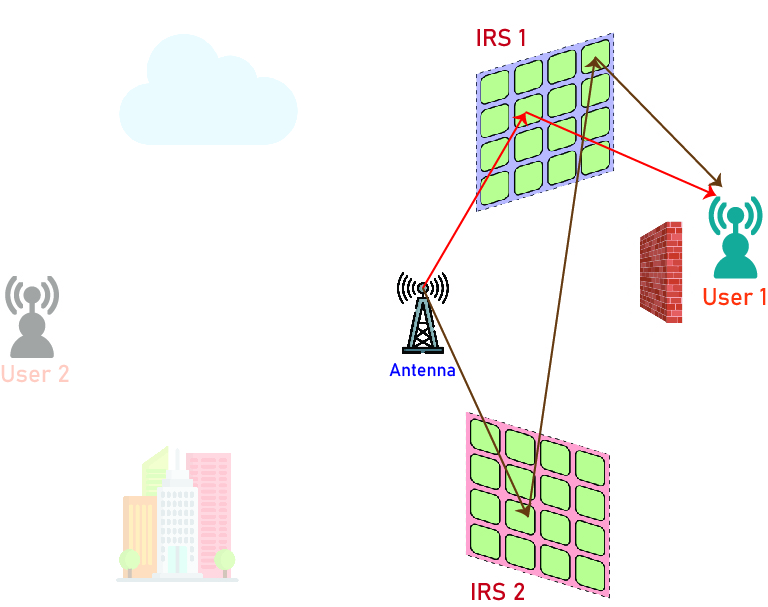
\includegraphics[scale=0.45]{with_obstacle__user1}
	
	\caption[سیگنال‌های دریافتی کاربر اول در شرایط با مانع]{
	سیگنال‌های دریافتی کاربر اول در شرایط با مانع
	}
%	\label{fig:fig-2_03}
\end{figure}

\begin{figure}[!h]
	\centering
	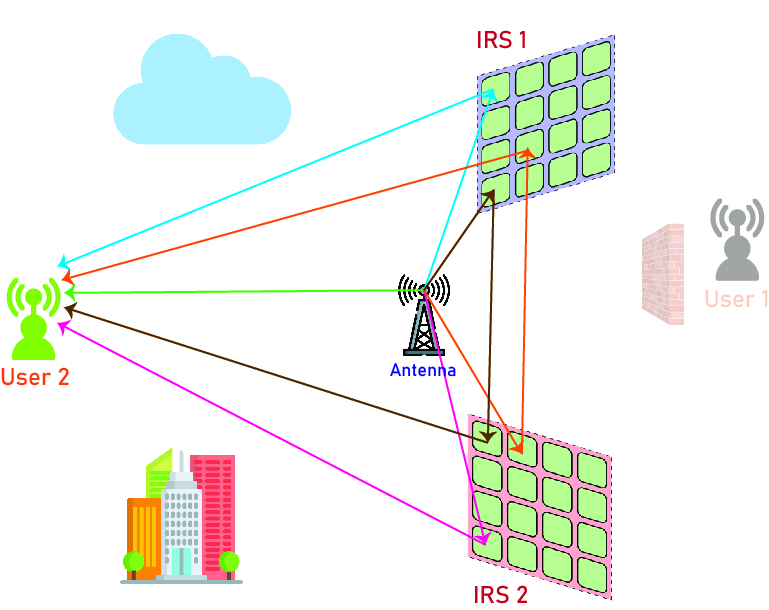
\includegraphics[scale=0.45]{with_obstacle__user2}
	
	\caption[سیگنال‌های دریافتی کاربر دوم در شرایط با مانع]{
		سیگنال‌های دریافتی کاربر دوم در شرایط با مانع
	}
%	\label{fig:fig-2_0}
\end{figure}
%%%%%%%%%%%%%%%%%%%%%%%%%%%%%%%%%%%%%%%%%%%
\newpage
\section{نوآوری ما}

در حال حاضر، همان‌طور که دیده‌اید، تعداد زیادی مقاله و مطلب در مورد مفهوم سطوح بازتابنده هوشمند وجود دارد. نه تنها تعداد اندکی از آن‌ها اثر بازتاب دوگانه یا بازتاب درجه دوم بین \lr{IRS} در کل عملکرد سیستم را در نظر گرفته‌اند، بلکه تقریباً تمامی آن‌ها اثر خط دید مستقیم (\lr{LoS}) را در این سناریوها با اعمال یک مانع نادیده گرفته‌اند. این نادیده‌گرفتن، انگیزه‌ای برای ما به وجود آورد تا یک سناریو را پیشنهاد دهیم تا اثر بازتاب دوگانه در حضور سیگنال‌های خط دید مستقیم را تجزیه و تحلیل کنیم. در این مقاله، به طور کلی، به تحلیل بهبودی که در حضور بازتاب دوگانه به دست می‌آید، می‌پردازیم تا ببینیم آیا اثر بازتاب دوگانه را می‌توان نادیده گرفت یا خیر.


\newpage
‌
\chapter{الگوریتم بهینه‌سازی}
در این فصل ابتدا سیستم مدل و چنل مدل را بیان میکنیم و سپس تکنیک ساده‌کردن مسئله به کمک متغیرهای واسط را شرح میدهیم. در ادامه، الگوریتم اصلی حل مسئله یعنی بهینه‌سازی دوره‌ای را مرور میکنیم و سپس دوگانه لاگرانژ و الگوریتم جستجوی ریشه دوبخشی را توضیح مختصری میدهیم و به کمک آنها، ضرایب آنتن را بهینه میکنیم. سپس ضرایب فاز را بکمک روش معروف گرادیان نزولی بهینه‌سازی کرده و در نهایت، 3 ناحیه اصلی بهینه‌سازی ضرایب فاز را شرح میدهیم. 
\newpage
%%%%%%%%%%%%%%%%%%%%%%%%%%%%%%%%%%%%%%%%%%%
\section{
	مدل سیستم و مدل کانال و مسئله بهینه‌سازی
}

\subsection{مدل سیستم}
طبق سناریویی که در فصل قبل شرح دادیم، سیگنال دریافتی در هر کاربر به شرح زیر می‌باشد:
\begin{equation}
	x = \sum_{k=1}^{K} w_k s_k, \label{eq:transmitted_signal}
\end{equation}
که دیتای کاربر \lr{k} ام توسط $s_k$ نمایش داده میشود. همچنین فرض میشود که این $s_k$ ها به ازای ($k = 1, \ldots, K$) متغیرهای رندوم و مستقل با میانگین صفر و واریانس 1 باشند.\\
از طرفی $w_k \in \mathbb{C}^{N_t \times 1}$ بردار ضرایب آنتن فرستنده هستند.\\
اکنون سیگنال دریافتی برای کاربر \lr{k} ام به شرح زیر قابل ساده‌سازی میباشد:
\begin{align*}
	y_k = &\underbrace{h_{d,k}^H x}_
	{\substack{\text{لینک مستقیم}}}
	\quad + \quad \\
	&\underbrace{h_{r_1,k}^H \Phi_1 G_1 x}_
	{\substack{\text{بازتاب مرتبه اول سطح هوشمند 1}}}
	\quad + \quad
	\underbrace{h_{r_2,k}^H \Phi_2 G_2 x}_
	{\substack{\text{بازتاب مرتبه اول سطح هوشمند 2}}}
	\quad + \quad \\ 
	&\underbrace{h_{r_1,k}^H \Phi_1 D \Phi_2 G_2 x}_
	{\substack{\text{بازتاب مرتبه دوم سطح هوشمند}}}
	\quad + \quad
	\underbrace{h_{r_2,k}^H \Phi_2 D^H \Phi_1 G_1 x}_
	{\substack{\text{بازتاب مرتبه دوم سطح هوشمند}}} \quad + \quad
	\underbrace{u_k}_
	{\substack{\text{نویز سفید گاوسی جمع‌شونده}}}
\end{align*}

بگونه‌ای که $u_k \sim \mathcal{CN}(0, \sigma_0^2)$ نشان‌دهنده نویز گاوسی در کاربر \lr{k} ام میباشد.
\newpage
اکنون به سراغ نوشتن نسبت سیگنال به نویز بعلاوه تداخل(\lr{SINR}) میرویم.\\
برای هر کاربر، نویز گاوسی بعلاوه سیگنال کاربران دیگر بعنوان سیگنال مزاحم تلقی شده و در مخرج کسر قرار میگیرند. پس \lr{SINR} کاربر \lr{k} به شکل زیر است:
\[
\gamma_k = \frac{{\left|\left(h_{d,k}^H + h_{r_1,k}^H \Phi_1 G_1 + h_{r_2,k}^H \Phi_2 G_2 + h_{r_1,k}^H \Phi_1 D \Phi_2 G_2 + h_{r_2,k}^H \Phi_2 D^H \Phi_1 G_1 \right)w_k\right|^2}}{{\sum_{i=1,i\neq k}^{K} \left|\left(h_{d,k}^H + h_{r_1,k}^H \Phi_1 G_1 + h_{r_2,k}^H \Phi_2 G_2 + h_{r_1,k}^H \Phi_1 D \Phi_2 G_2 + h_{r_2,k}^H \Phi_2 D^H \Phi_1 G_1 \right)w_i\right|^2 + \sigma^2_0}}
\]
همچنین شرط توان نیز برای مجموع کاربران به‌شکل زیر نوشته میشود:
\[
\sum_{k=1}^{K} ||w_k||^2 \leq P_T
\]
بگونه‌ای که:
$\mathbf{W} = [\mathbf{w}_1, \mathbf{w}_2, \ldots, \mathbf{w}_K] \in \mathbb{C}^{N_t \times K}$

\subsection{مدل کانال}
برای مدل کردن کانال، ابتدا از مدل‌های رندوم استفاده مینماییم اما در صورت جواب گرفتن از الگوریتم، آن‌را برای مدل‌های رایلی و رایسی نیز بهینه‌سازی میکنیم.

\subsection{مسئله بهینه‌سازی}
در این پروژه، هدف، بیشینه‌کردن مجموع نرخ دریافتی کاربران است که به آن \lr{WSR} گفته میشود. برای اینکار میبایست ضرایب آنتن و ضرایب فاز سطوح هوشمند را بصورت همزمان و توام بهینه‌سازی نماییم زیرا این دو دسته از متغیرها بر یکدیگر تاثیر میگذارند و نمیتوانند بصورت جداگانه بهینه‌سازی شوند. همچنین باید هر جوابی که برای ضرایب آنتن ارائه میشود، در شرط توان صدق نماید. پس مسئله را میتوان به شکل زیر فرموله کرد:
\begin{align*}
	(P1) \quad \max_{\mathbf{W}, \boldsymbol{\Phi_1}, \boldsymbol{\Phi_2}} \quad & f_1(\mathbf{W}, \boldsymbol{\Phi_1}, \boldsymbol{\Phi_2}) = \sum_{k=1}^{K} \omega_k \log_2(1 + \gamma_k) \\
	\text{به شرط} \quad & \theta_{m_k} \in \mathcal{F}, \quad \forall m_k = 1, \ldots, M_k, \tag{4-2} \\
	& \sum_{k=1}^{K} \| \mathbf{w}_k \|_2^2 \leq P_T,
\end{align*}

%%%%%%%%%%%%%%%%%%%%%%%%%%%%%%%%%%%%%%%%%%%
\section{الگوریتم بهینه‌سازی متناوب}
در این بخش، الگوریتم \lr{Alternating optimization} 
\cite{13}, \cite{14}
یا بهینه‌سازی پی‌در‌پی که به الگوریتم \lr{Coordinate Descent } یا مختصات نزولی نیز معروف میباشد را تعریف و نحوه بکارگیری آنرا شرح خواهیم داد.
\subsection{تعریف}
الگوریتم‌های هماهنگ نزولی مسائل بهینه‌سازی را با حداقل‌سازی تقریبی در امتداد جهت‌های مختصاتی یا ابرصفحه مختصاتی حل می‌کنند. این روش سال‌هاست که در برنامه‌های کاربردی مورد استفاده قرار می‌گیرد و محبوبیت آن‌ به دلیل مفید بودنش در تجزیه و تحلیل داده‌ها، یادگیری ماشین و دیگر زمینه‌های مورد علاقه فعلی، همچنان در حال رشد است.

\subsection{استفاده}
در مسئله بهینه‌سازی فعلی، 2 دسته اصلی پارامتر داریم که باید بهینه‌سازی شوند. دسته اول مربوط به ضرایب آنتن میباشد که یک بردار با طول مشخص است. دسته دوم مربوط به ضرایب سطوح هوشمند است که خود به 2 دسته تقسیم میشوند زیرا 2 سطح هوشمند مستقل از هم داریم. البته لازم به ذکر است که در ادامه و با بوجود آمدن متغیرهای کمکی در طول مسئله، این دسته از متغیرها نیز به پارامترهای بهینه‌سازی اضافه میشوند که طول عمر آنها بصورت محلی تعریف میشود و جزو پارامترهای اصلی مسئله نیستند.

پس به طول کلی یک حلقه داریم که ابتدا ضرایب اولیه‌ای را برای فاز سطوح هوشمند در نظر گرفته و ضرایب آنتن‌ را بهینه‌سازی مینماییم. سپس ضرایب آنتن را ثابت فرض کرده و ضرایب سطوح هوشمند را بهینه‌سازی مینماییم.
\begin{figure}[!h]
	\centering
	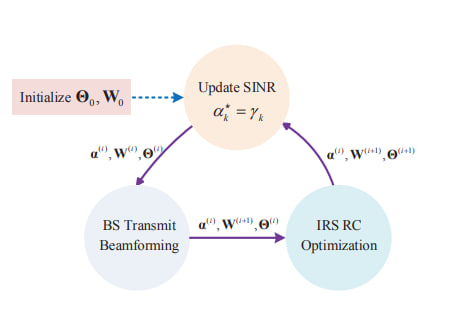
\includegraphics[scale=0.65]{AO}
	
	\caption[شیوه استفاده الگوریتم مختصات نزولی در پروژه]{
		شیوه استفاده الگوریتم مختصات نزولی در پروژه
	}
	%	\label{fig:fig-2_03}
\end{figure}
%%%%%%%%%%%%%%%%%%%%%%%%%%%%%%%%%%%%%%%%%%%
\section{تبدیل دوگان لاگرانژی}
یکی از مشکلاتی که در این مسئله بهینه‌سازی و همه مسائل مرتبط با بهینه‌سازی حداکثر نرخ قابل‌دسترسی با آن روبرو هستیم، وجود تابع لاگاریتم میباشد. اگر فقط یک عدد تابع لگاریتم وجود داشت، به علت اینکه لگاریتم تابعی اکیدا یکنوا (اکیدا صعودی) است، میتوانستیم آن را حذف کرده و فقط تابع جلوی لگاریتم را بهینه‌سازی نماییم اما در اینجا با جمع چند لگاریتم روبرو هستیم. شاید یک راه حل احتمالی این باشد که از قانون تبدیل جمع به ضرب در لگاریتم استفاده شود اما این خود باعث افزایش پیچیدگی مسئله میشود. 
\subsection{تعریف}
اکنون که مشکل را درک کردیم، به سراغ معروف‌ترین راه‌حل آن میرویم. یکی از تبدیل‌هایی که میتوان جهت حذف لگاریتم در چنین مسائلی استفاده نمود، تبدیل دوگانی لاگرانژ لگاریتمی میباشد. 
این تبدیل توسط دو عضو جامعه علمی برق در سال 2018 در بخش دوم مقاله‌ای جهت استفاده برای حل مسائل مخابرات ارائه گردید.

تکنیک به گونه‌ای میباشد که با اضافه کردن پارامترهایی اختیاری به نام آلفا به مسئله، باعث جابجایی تابع جلوی لگاریتم به بیرون آن میشود و عملا با حذف لگاریتم، باعث ساده‌شدن مسئله بهینه‌سازی میشود. در ادامه از این تکنیک پرکاربرد استفاده خواهیم‌نمود.
\subsection{ساده‌سازی مسئله}
این تکنیک در مسئله ما به‌صورت زیر قابل استفاده میباشد:
\[
f_{1a}(\mathbf{W}, \boldsymbol{\Theta}, \boldsymbol{\alpha}) = \sum_{k=1}^{K} \omega_k \log_2(1 + \alpha_k) - \sum_{k=1}^{K} \omega_k \alpha_k + \sum_{k=1}^{K} \frac{\omega_k (1 + \alpha_k) \gamma_k}{1 + \gamma_k}
\]
همانطور که مشاهده میشود، مسئله 4-2 قابل تبدیل به مسئله بالا میباشد که پارامتر اختیاری آلفا به تعداد کاربران به مسئله اضافه شده‌است.

همچنین گاما همان نسبت سیگنال به نویز معروف میباشد.
اکنون شاید این سوال پیش بیاید که آیا با اضافه‌شدن یک دسته پارامتر جدید، چگونه باعث ساده‌تر شدن مسئله میشویم؟

جواب این سوال وقتی مشخص میشود که به کمک الگوریتم مختصات نزولی شروع به بهینه‌سازی این دو دسته پارامتر نماییم:

1- دسته اول همان پارامترهای آنتن و سطوح هوشمند

2- دسته دوم پارامترهای اختیاری اضافه‌شده به مسئله

برای اینکار، ابتدا پارامترهای دسته اول را ثابت فرض میکنیم و نسبت به پارامترهای دسته دوم مشتق میگیریم.
نکته قابل‌توجه اینکه این مشتق‌گیری به سادگی قابل انجام است و با صفر قرار دادن آن، مقدار بهینه آلفا به شکل زیر یافت میشود:

 \[\alpha_k^\circ = \gamma_k\]

 اکنون با ثابت فرض کردن آلفا، مسئله به شکل زیر تبدیل میشود و به سراغ بهینه‌سازی پارامترهای دسته اول میرویم :
 
 \[
 (P1'') \quad \max \mathbf{W}, \boldsymbol{\Theta} \quad \sum_{k=1}^{K} \frac{\alpha_k^\sim \gamma_k}{1 + \gamma_k}
 \]
 
 بگونه‌ای که $\alpha_k^\sim = \omega_k(1 + \alpha_k)$ میباشد.
 
 اکنون به مجموع چند عبارت کسری رسیدیم که در ادامه با استفاده از تکنیک برنامه‌ریزی چند کسری به حل این مسئله میپردازیم.
%%%%%%%%%%%%%%%%%%%%%%%%%%%%%%%%%%%%%%%%%%%
\section{برنامه‌ریزی چند کسری}
\cite{12}
اکنون با چند کسر مواجه هستیم که مشتق‌گرفتن از آنها و حل معادله حاصله به راحتی امکان‌پذیر نیست. پس لازم است از تبدیل دیگری به‌نام برنامه‌ریزی چند کسری استفاده نماییم تا این مسئله به فرم خطی تبدیل شود بگونه‌ای که مسئله حاصله، معادل مسئله اصلی باشد یعنی نقاط بهینه یکسانی داشته باشند. 

\subsection{تعریف}
این تبدیل در بخش اول مقاله‌ای که در بخش قبل به آن اشاره شد معرفی شده‌است. همانند تبدیل معرفی شده در بخش قبل و سایر تبدیل‌ها، یک دسته پارامتر اختیاری بنام بتا به مسئله اضافه میشوند که البته باعث ساده‌شدن مسئله بهینه‌سازی میشود.\\
در ادامه به نحوه استفاده از این تکنیک در مسئله میپردازیم.
\subsection{ساده‌سازی مسئله}
ابتدا برای ساده‌سازی نوشتار، یک پارامتر جدید مربوط به کانال‌ها تعریف میکنیم:
\[\mathbf{h}_k = \mathbf{h}_d,k + \mathbf{GH}\boldsymbol{\Theta}\mathbf{h}_r,k\]
پس نسبت سیگنال به نویز به شکل زیر تغییر میکند:
\[
\gamma_k = \frac{{\lVert \mathbf{h}_k \mathbf{w}_k \rVert^2}}{{\sum_{i=1,i\neq k}^{K} \lVert \mathbf{h}_k \mathbf{w}_i \rVert^2 + \sigma_0^2}}
\]
اکنون با استفاده از تبدیل کسری و اضافه شدن پارامتر بتا، مسئله بهینه‌سازی به شکل زیر تغییر میکند و به فرم خطی نوشته می‌شود:
\[
f2a(\mathbf{W}, \boldsymbol{\beta}) = \sum_{k=1}^{K} 2 \sqrt{\alpha_k^\sim} \Re \left\{ \beta_k^* \mathbf{h}_k^H \mathbf{w}_k \right\} - \sum_{k=1}^{K} \lvert \beta_k \rvert^2 \sum_{i=1}^{K} \lVert \mathbf{h}_k \mathbf{w}_i \rVert^2 + \sigma_0^2.
\]
بگونه‌ای که دامنه بتا برابر اعداد مختلط باشد.
%%%%%%%%%%%%%%%%%%%%%%%%%%%%%%%%%%%%%%%%%%%
\section{بهینه‌سازی ضرایب آنتن}
اکنون دوباره با بکارگیری الگوریتم مختصات نزولی یا \lr{Coordinate Descent} میتوان پارامتر های بتا و سایر پارامترها را در داخل یک حلقه، بهینه‌سازی کرد.\\
برای اینکار میبایست ابتدا نسبت به بتا مشتق گرفته و مقدار بهیه آن را بدست آوریم. این کار به سادگی قابل انجام است. 

\subsection{مقدار بتا بهینه}
مقدار بهینه بتا در زیر آورده شده‌است:
\[
\beta_k^* = \sqrt{\alpha_k^\sim} \frac{{\mathbf{h}_k^H \mathbf{w}_k}}{{\sum_{i=1}^{K} \lVert \mathbf{h}_k \mathbf{w}_i \rVert^2 + \sigma_0^2}}.
\]
\subsection{مقدار بهینه بردار آنتن}
اکنون نوبت به بهینه‌سازی اولین دسته پارامتر اصلی مسئله یعنی ضرایب فعال آنتن رسیده است. همانند سایر پارامترها برای بدست آوردن مقدار بهینه آن، نسبت به \lr{W} مشتق گرفته و برابر صفر قرار میدهیم. نتیجه در رابطه زیر قابل مشاهده‌است:
\[\mathbf{w}_k^* = \sqrt{\alpha_k^\sim} \beta_k \left( \lambda_0 \mathbf{I}_M + \sum_{i=1}^{K} \lvert \beta_i \rvert^2 \mathbf{h}_i \mathbf{h}_i^H \right)^{-1} \mathbf{h}_k,
\]
البته لازم به ذکر است چون بر روی این دسته پارامتر، شرط توان نیاز است رعایت شود باید یک پارامتر کمکی به نام لامبدا به مسئله اضافه کنیم که با تغییر آن، شرط توان را برقرار سازیم.
مقدار لامبدا به صورت بهینه توسط حل نامعادله زیر بدست می‌آید:
\[
\lambda_0^* = \min \left( \lambda_0 \geq 0 : \sum_{k=1}^{K} \lVert \mathbf{w}_k \rVert^2 \leq PT \right).
\]
روش حل این نامعادله را توسط سریع‌ترین روش یعنی جستجوی دوبخشی در زیر توضیح خواهیم داد. 
\subsection{روش جستجوی دوبخشی}
یکی از ساده‌ترین و در عین حال بهینه‌ترین روش‌های جستجوی ریشه تابع در یک بازه، روش جستجوی دو بخشی یا \lr{Bisection Search}
میباشد. این روش میتواند به طور همزمان فقط یک ریشه را در یک بازه مشخص پیدا کند. برای اطمینان از وجود ریشه در یک بازه، طبق قضیه مقدار میانی، مقدار تابع باید در ابتدا و انتهای بازه مختلف‌العلامه باشند. این روش ابتدا وسط بازه را به عنوان نقطه سوم در نظر گرفته و مقدار آن را در تابع حساب میکند. سپس بازه جستجوی جدید بین نقطه سوم و نقطه‌ایست که علامت متفاوتی با نقطه سوم دارد. به همین روش بازه جستجو را کوچک کرده و در نهایت با یک شرط پایان مثلا تعیین شرط میزان خطا بر روی ریشه، الگوریتم متوقف میشود.

\subsection{حد بالای لامبدا}
یکی از مسائلی که در روش دو بخشی باید پیش از اجرای الگوریتم تعیین کنیم، نقطه شروع و پایان الگوریتم میباشد. نقطه شروع برای این مسئله همیشه از صفر میباشد اما حد بالای آن چگونه یافت میشود؟

- یک روش آنست که مقداری بسیار بزرگ برای آن قرار دهیم که اتفاقا در اکثر سناریوها روشی قابل انجام است اما به علت محاسبات سنگین‌تر با اعداد بزرگتر، باعث کند شدن الگوریتم و به علت بزرگ‌ بودن بازه جستجو، دیرتر به ریشه تابع همگرا میشود.

- اما در روش دوم، طبق مقاله [] میتوان از ضابطه زیر جهت حد بالای پارامتر لامبدا استفاده نمود:
\[
	g(\lambda) \leq \sum_{k=1}^{K}\left|\alpha_{k}\right|^{2}\left|q_{k}\right|^{2} \sum_{i=1}^{N} \frac{\left[\mathbf{Z}_{k}\right]_{i, i}}{\lambda_{\max }^{2}} \triangleq P_{\max }, \\
	\Rightarrow \lambda_{\max }=\sqrt{\frac{\sum_{k=1}^{K}\left|\alpha_{k}\right|^{2}\left|q_{k}\right|^{2} \sum_{i=1}^{N}\left[\mathbf{Z}_{k}\right]_{i, i}}{P_{\max }} .}
\]
از طریق روابط زیر نیز قابل اثبات است:
\[
	g(\lambda)  =\sum_{k=1}^{K}\left\|\mathbf{w}_{k}\right\|_{2}^{2}=
\]
\[
\sum_{k=1}^{K} \operatorname{Tr}\left(\mathbf{F}_{1}\left(\boldsymbol{\Sigma}_{1}+\lambda \mathbf{I}\right)^{-1} \mathbf{F}_{1}^{H} \alpha_{k} q_{k} \overline{\mathbf{h}}_{k} u_{k} u_{k}^{H} \overline{\mathbf{h}}_{k}^{H} q_{k} \alpha_{k} \mathbf{F}_{1}\left(\boldsymbol{\Sigma}_{1}+\lambda \mathbf{I}\right)^{-1} \mathbf{F}_{1}^{H}\right)=
\]
\[
	 \sum_{k=1}^{K}\left|\alpha_{k}\right|^{2}\left|q_{k}\right|^{2} \operatorname{Tr}\left(\left(\boldsymbol{\Sigma}_{1}+\lambda \mathbf{I}\right)^{-2} \mathbf{F}_{1}^{H} \overline{\mathbf{h}}_{k} u_{k} u_{k}^{H} \overline{\mathbf{h}}_{k}^{H} \mathbf{F}_{1}\right) \\
	 =\sum_{k=1}^{K}\left|\alpha_{k}\right|^{2}\left|q_{k}\right|^{2} \sum_{i=1}^{N} \frac{\left[\mathbf{Z}_{k}\right]_{i, i}}{\left(\varepsilon_{i}+\lambda\right)^{2}},
\]
%%%%%%%%%%%%%%%%%%%%%%%%%%%%%%%%%%%%%%%%%%%
\section{بهینه‌سازی ضرایب فاز سطوح هوشمند}
اکنون سراغ بهینه‌سازی دسته دوم از پارامترهای اصلی مسئله میرویم. دوباره برای تبدیل کسر به عبارتی خطی، نیاز است از برنامه‌ریزی چند کسری استفاده نماییم که در زیر قابل مشاهده است(اینبار با پارامتر اپسیلون این کار را انجام میدهیم):
\[
	f_{3 a}(\boldsymbol{\theta}, \boldsymbol{\varepsilon})=  \sum_{k=1}^{K} 2 \sqrt{\tilde{\alpha}_{k}} \operatorname{Re}\left\{\varepsilon_{k}^{*} \boldsymbol{\theta}^{\mathrm{H}} \mathbf{a}_{k, k}+\varepsilon_{k}^{*} b_{k, k}\right\} \\
	 -\sum_{k=1}^{K}\left|\varepsilon_{k}\right|^{2}\left(\sum_{i=1}^{K}\left|b_{i, k}+\boldsymbol{\theta}^{\mathrm{H}} \mathbf{a}_{i, k}\right|^{2}+\sigma_{0}^{2}\right)
\]

\subsection{مقدار اپسیلون بهینه}
همانند بخش قبل که مقدار بهینه بتا را بدست آوردیم، اکنون به سراغ محاسبه مقدار بهینه اپسیلون میرویم:\
\[
\varepsilon_{k}^{\circ}=\frac{\sqrt{\tilde{\alpha}_{k}}\left(b_{k, k}+\boldsymbol{\theta}^{\mathrm{H}} \mathbf{a}_{k, k}\right)}{\sum_{i=1}^{K}\left|b_{i, k}+\boldsymbol{\theta}^{\mathrm{H}} \mathbf{a}_{i, k}\right|^{2}+\sigma_{0}^{2}} .
\]
\newpage
\subsection{روش گرادیان نزولی}
\cite{15}
این الگوریتم بهینه‌سازی، در عین مفهوم بسیار ساده‌ای که دارد، یک روش بسیار پرکاربرد و در صورت انتخاب کردن طول گام مناسب، بسیار سریع است.\\
برای پیدا کردن کمینه محلی، کافیست تابع مشتق‌پذیر باشد تا از آن مشتق گرفته و در جهت خلاف آن حرکت نماییم. 
برای پیدا کردن بیشینه، کافیست در جهت مشتق حرکت نماییم.
لازم به ذکر است که همه الگوریتم‌ها نقاط بهینه‌ محلی میدهند و اگر تابع محدب باشد، آن نقطه بهینه محلی، بهینه سراسری نیز می‌باشد.\\
در این روش نیاز به انتخاب طول گام داریم که سرعت همگرایی را مشخص می کند. اگر طول گام خیلی کوچک باشد، ممکن است دیر همگرا شود. اگر طول گام خیلی بزرگ انتخاب شود، ممکن است در بهینه محلی گیر نکند. پس باید مقداری مناسب برای آن قرار دهیم که روش‌های زیادی نیز برای انتخاب طول گام به شکلی تطبیق‌پذیر یا \lr{adaptive} نوشته شده‌است.

\newpage
\subsection{ضرایب بهینه سطوح هوشمند یک و دو}
برای محاسبه مقدار بهینه تتا میتوان دوباره مشتق گرفت ولی این روش سرعت کمی دارد و بهتر است از روش گرادیان نزولی برای یک بردار استفاده نماییم.

ابتدا چند تعریف ساده ارائه میدهیم:
\[
	\left|b_{i, k}+\boldsymbol{\theta}^{\mathrm{H}} \mathbf{a}_{i, k}\right|^{2}  =\left(b_{i, k}+\boldsymbol{\theta}^{\mathrm{H}} \mathbf{a}_{i, k}\right)\left(b_{i, k}^{*}+\mathbf{a}_{i, k}^{\mathrm{H}} \boldsymbol{\theta}\right) \\
	 =\boldsymbol{\theta}^{\mathrm{H}} \mathbf{a}_{i, k} \mathbf{a}_{i, k}^{\mathrm{H}} \boldsymbol{\theta}+2 \operatorname{Re}\left\{b_{i, k}^{*} \boldsymbol{\theta}^{\mathrm{H}} \mathbf{a}_{i, k}\right\}+\left|b_{i, k}\right|^{2}
\]
\[	f_{4}(\boldsymbol{\theta})  =f_{3 a}\left(\boldsymbol{\theta}, \boldsymbol{\varepsilon}^{\circ}\right) \\
	 =-\boldsymbol{\theta}^{\mathrm{H}} \boldsymbol{R} \boldsymbol{\theta}+2 \operatorname{Re}\left\{\boldsymbol{\theta}^{\mathrm{H}} \boldsymbol{e}\right\}+C,
\]
\[	\boldsymbol{R}  =\sum_{k=1}^{K}\left|\varepsilon_{k}\right|^{2} \sum_{i=1}^{K} \mathbf{a}_{i, k} \mathbf{a}_{i, k}^{\mathrm{H}},
\]
\[
	\boldsymbol{e}  =\sum_{k=1}^{K}\left(\sqrt{\tilde{\alpha}_{k}} \varepsilon_{k}^{*} \mathbf{a}_{k, k}-\left|\varepsilon_{k}\right|^{2} \sum_{i=1}^{K} b_{i, k}^{*} \mathbf{a}_{i, k}\right),
\]
\[
	C  =\sum_{k=1}^{K}\left(2 \sqrt{\tilde{\alpha}_{k}} \operatorname{Re}\left\{\varepsilon_{k}^{*} b_{k, k}\right\}-\left|\varepsilon_{k}\right|^{2}\left(\sigma_{0}^{2}+\sum_{i=1}^{K}\left|b_{i, k}\right|^{2}\right)\right)
\]

ابتدا به کمک گرادیان نزولی و مپ کردن جواب بر روی دایره واحد، مقدار گرادیان را از طریق رابطه زیر محاسبه میکنیم:
\[
\nabla_{\Theta} f_{4}=2 \operatorname{Re}\left\{(\mathbf{R \theta}-\mathbf{e})^{*} \odot(-j \mathbf{\theta})\right\},
\]
اکنون به کمک مفهوم روش \lr{iterative} گرادیان نزولی، مقدار جدید ضرایب فاز سطح هوشمند شماره 1 را از ترکیب مقدار قبلی بهمراه ضریبی از تغییرات (گرادیان) توسط رابطه زیر بدست می‌آوریم:
\[
\boldsymbol{\Theta}^{(t+1)}=\boldsymbol{\Theta}^{(t)}-\gamma^{(t)} \nabla_{\boldsymbol{\Theta}} f\left(\mathbf{X}^{(t)}\right),
\]
محاسبه ضرایب سطح هوشمند شماره 2 نیز به روش مشابه قابل انجام است.
\newpage
\subsection{سه ناحیه اصلی بهینه‌سازی ضرایب فاز}
برای بهینه‌سازی ضرایب فاز، 3 ناحیه اصلی وجود دارد که جواب نهایی را میتوان به آن ناحیه مپ کرد.

- ناحیه اول، ناحیه درون دایره واحد است که اکثر الگوریتم‌ها بصورت پیش‌فرض جواب را در این ناحیه میدهند. این ناحیه الزاما جواب بهینه سراسری نمیدهد زیرا همراه با کاهش توان همراه است (اندازه بردار داخل دایره واحد کمتر از 1 میباشد). 

- ناحیه دوم، ناحیه روی دایره یکه است. احتمال وجود بهینه‌ سراسری در این ناحیه بالا است. جواب های درون دایره واحد که از الگوریتم‌های مرحله قبل بدست می‌آید، به این ناحیه مپ میشوند یعنی اندازه بردار آنها برابر واحد میشود یا به عبارتی آن عدد مختلط را بر اندازه‌اش تقسیم میکنند.

- ناحیه سوم که ناحیه ایست که عملا کاربرد واقعی دارد، ناحیه کوانتیزه‌شده روی دایره یکه است. به عبارتی این ناحیه زیرمجموعه ناحیه قبل است و فقط شامل نقاط محدودی از آن میشود.  مثلا می‌توان کوانتیزیشن 9 بیتی انجام داد که حدودا خطای یک درجه می‌دهد.

این مسئله بر روی ناحیه دوم حل شده است که به راحتی موقع پیاده‌سازی میتواند به نزدیک‌ترین نقطه در ناحیه سوم مپ شود.
%%%%%%%%%%%%%%%%%%%%%%%%%%%%%%%%%%%%%%%%%%%
\newpage
‌
\chapter{نتایج و پیشنهادات}
در این فصل ابتدا نتایج حاصل از پیاده‌سازی الگوریتم توضیح داده‌شده در فصل قبل را برای هر دو سناریو مورد بررسی قرار میدهیم و سپس به دو مورد از کارهایی که در آینده برای پیشبرد این تحقیق و کمک به سایر محققان قابل انجام است اشاره میکنیم.
\newpage
%%%%%%%%%%%%%%%%%%%%%%%%%%%%%%%%%%%%%%%%%%%
\section{نتایج}
در این بخش، سناریو را در 2 حالت بدون مانع و همراه با مانع شبیه‌سازی میکنیم. جهت اینکار، پارامترهای لازم در این شبیه‌سازی را مطابق مقادیر زیر قرار داده و برای \lr{M1} هایی که مضرب 10 هستند و برای هر \lr{M1} 10 بار شبیه‌سازی را اجرا کرده و مقادیر را درونیابی میکنیم تا به نمودارهای زیر برسیم.
مقادیر قرار داده‌شده در شبیه‌سازی به شرح زیر است:

	- تعداد المان‌های آنتن: 20 = \lr{N}
	
	- تعداد المان‌های سطح هوشمند دوم: 20 = \lr{M2}
	
	- وزن نرخ هر کاربر: 1
	
	- مجموع توان دو کاربر: 10 میلی وات
	
	- انحراف از معیار نویز: \lr{0.0001}
	
	- ضریب افت توان مسیر دید مستقیم: \lr{2.5}
	
	- ضریب افت توان مسیر بین آنتن و سطوح هوشمند یا سطوح هوشمند و کاربر: 2
	
	- ضریب افت توان مسیر بین سطوح هوشمند: \lr{1.8}
	
	- فاصله‌ کاربر 1 تا آنتن: 50 متر
	
	- فاصله‌ کاربر 2 تا آنتن: 60 متر
	
	- فاصله سطح هوشمند 1 تا آنتن: 20 متر
	
	- فاصله سطح هوشمند 2 تا آنتن: 30 متر
	
	- فاصله کاربر 1 تا سطح هوشمند 1: 50 متر

	- فاصله کاربر 1 تا سطح هوشمند 2: 30 متر
	
	- فاصله کاربر 2 تا سطح هوشمند 1: 40 متر
	
	- فاصله کاربر 2 تا سطح هوشمند 2: 20 متر
	
	- فاصله بین سطوح هوشمند: 40 متر
	
	- طول گام الگوریتم گرادیان نزولی: \lr{0.1}
	
%%%%%%%%%%%%%%%%%%%%%%%%%%%%%%%%%%%%%%%%%%%
\newpage
\subsection{نتایج و تحلیل بهینه‌سازی بدون مانع}
طبق شرایط بالا و در حالت بدون مانع، شبیه‌سازی را اجرا کرده و نمودارهای زیر برای نرخ کاربر 1، کاربر 2 و مجموع نرخ هر دو کاربر رسم‌ شده است:

\begin{figure}[!h]
	\begin{minipage}{0.5\textwidth}
		\centering
		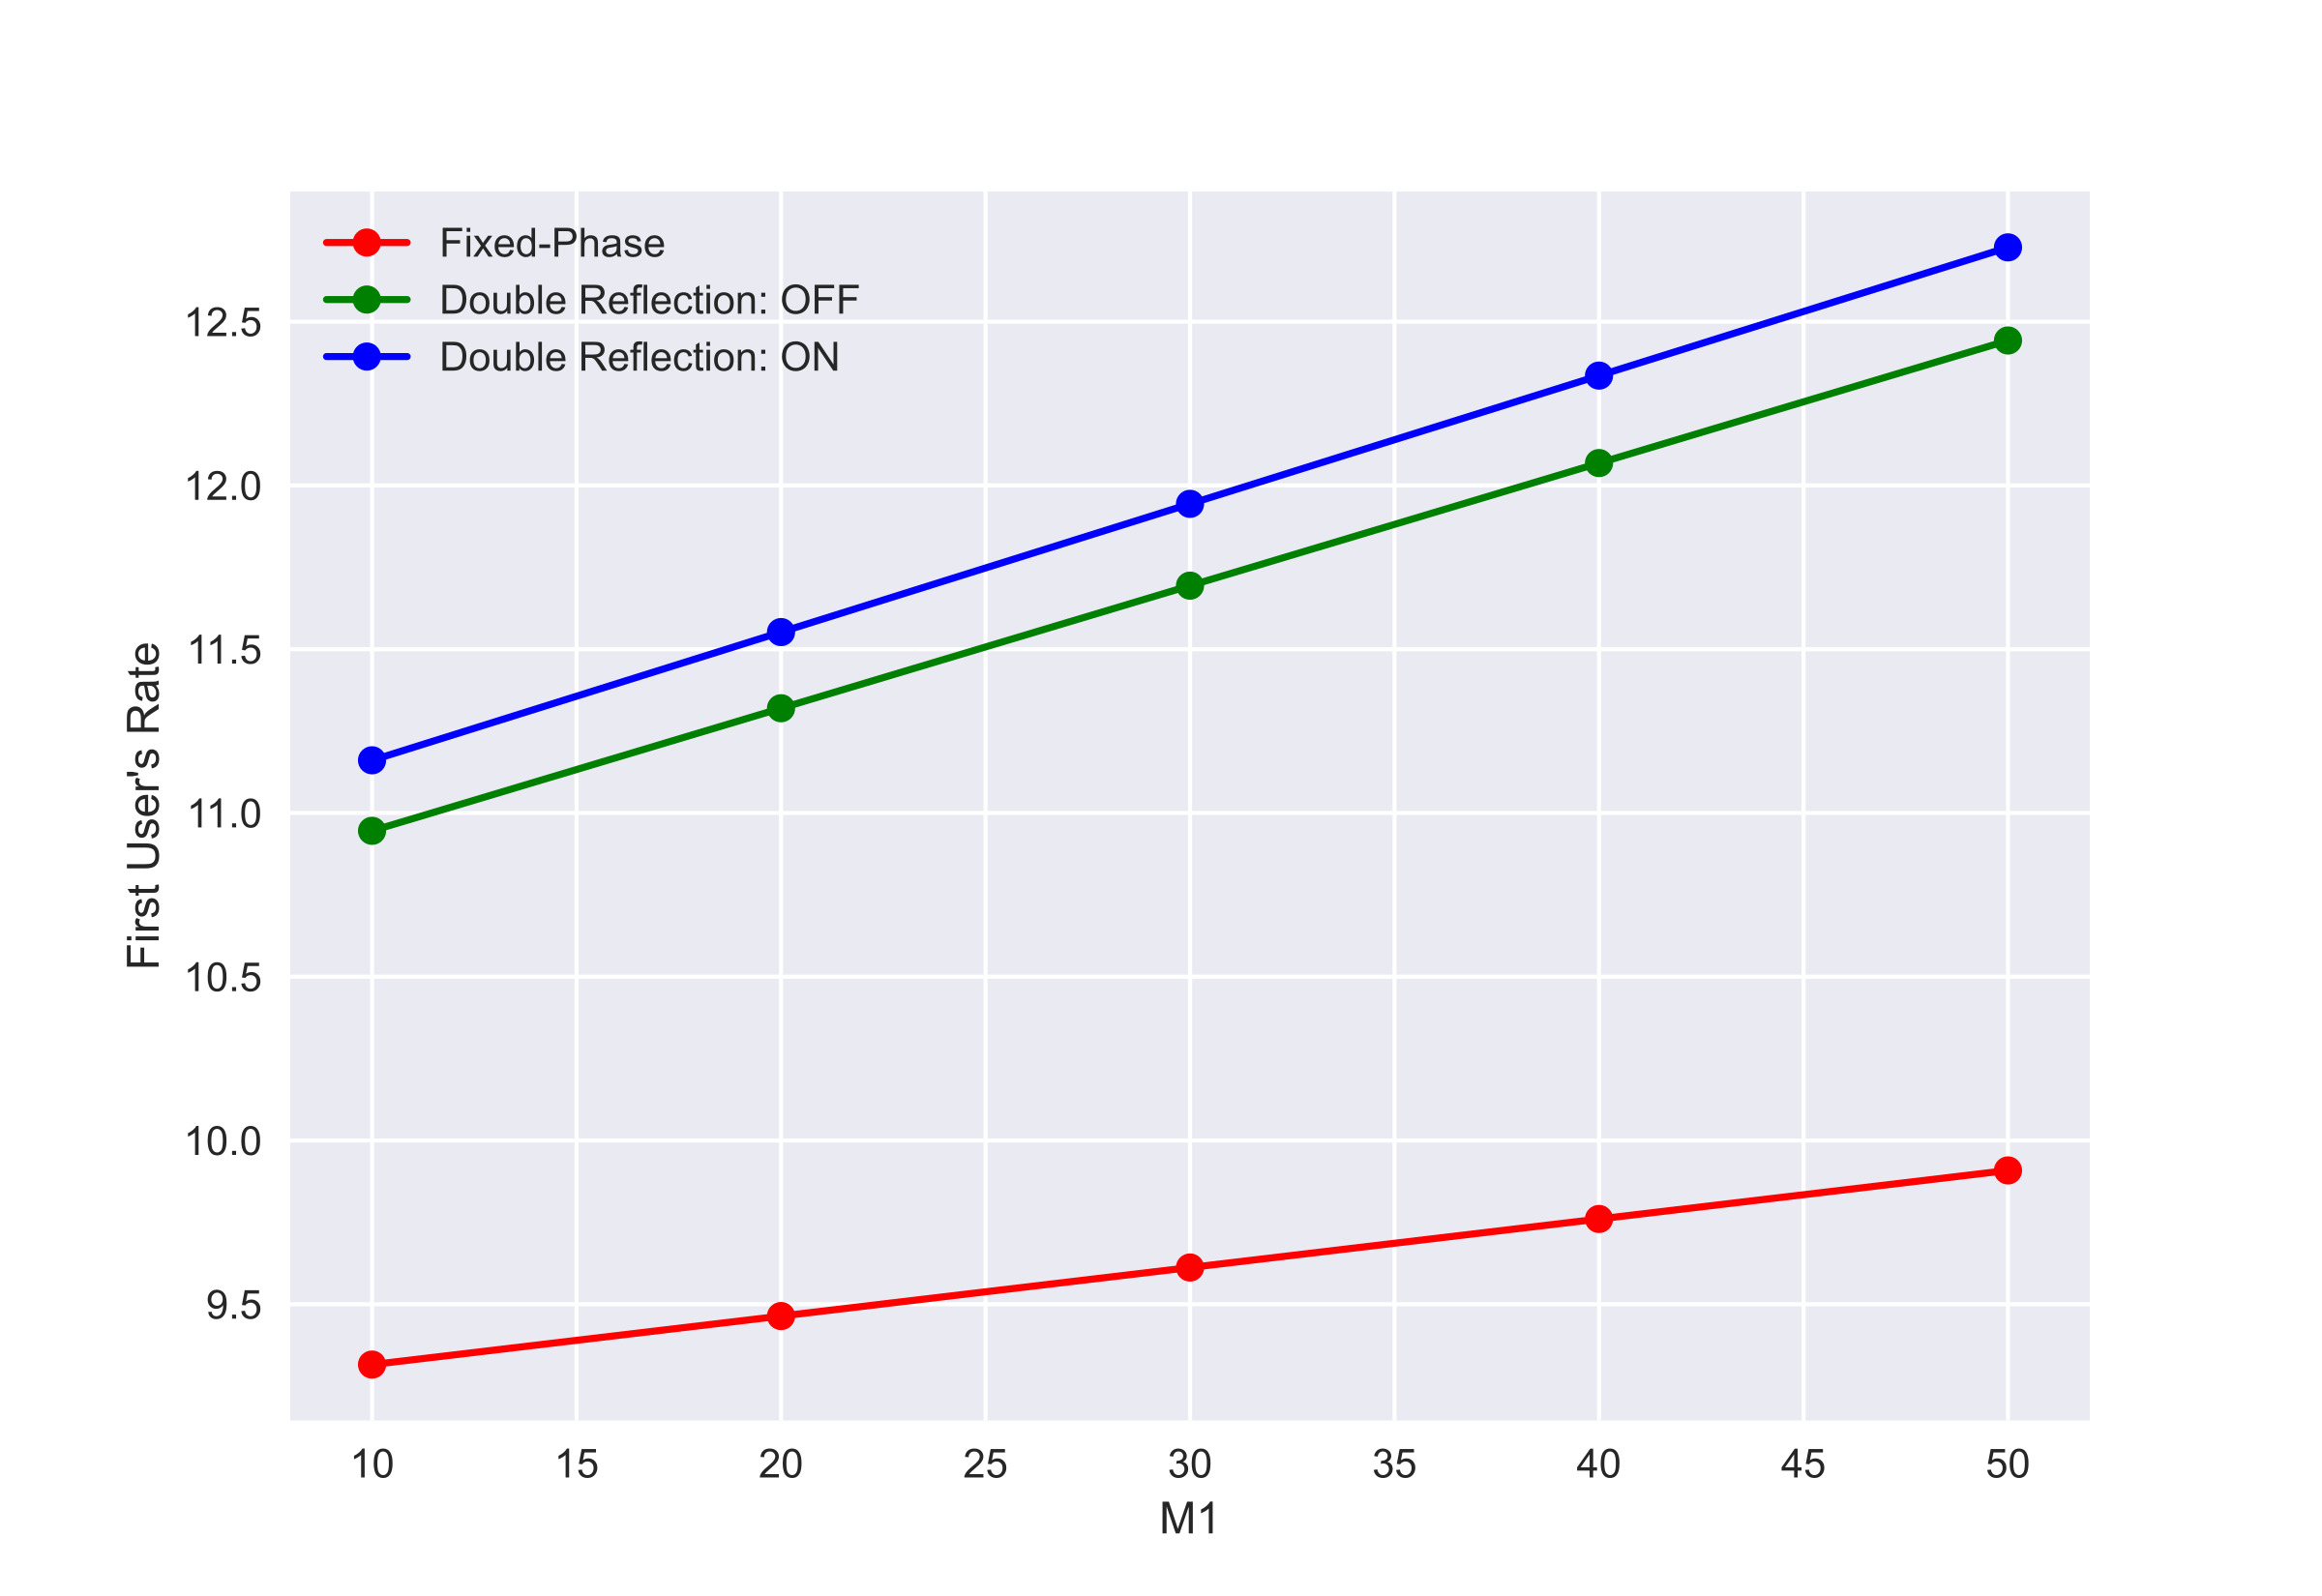
\includegraphics[scale=0.1]{No Blockage First User's Rate}
		\captionsetup{width=0.8\linewidth}
		\caption[
		نرخ کاربر اول در شرایط بدون مانع
		]{
			نرخ کاربر اول در شرایط بدون مانع
		}
%		\label{fig:Picture-2_06}
	\end{minipage}
	\hfill
	\begin{minipage}{0.5\textwidth}
		\centering
		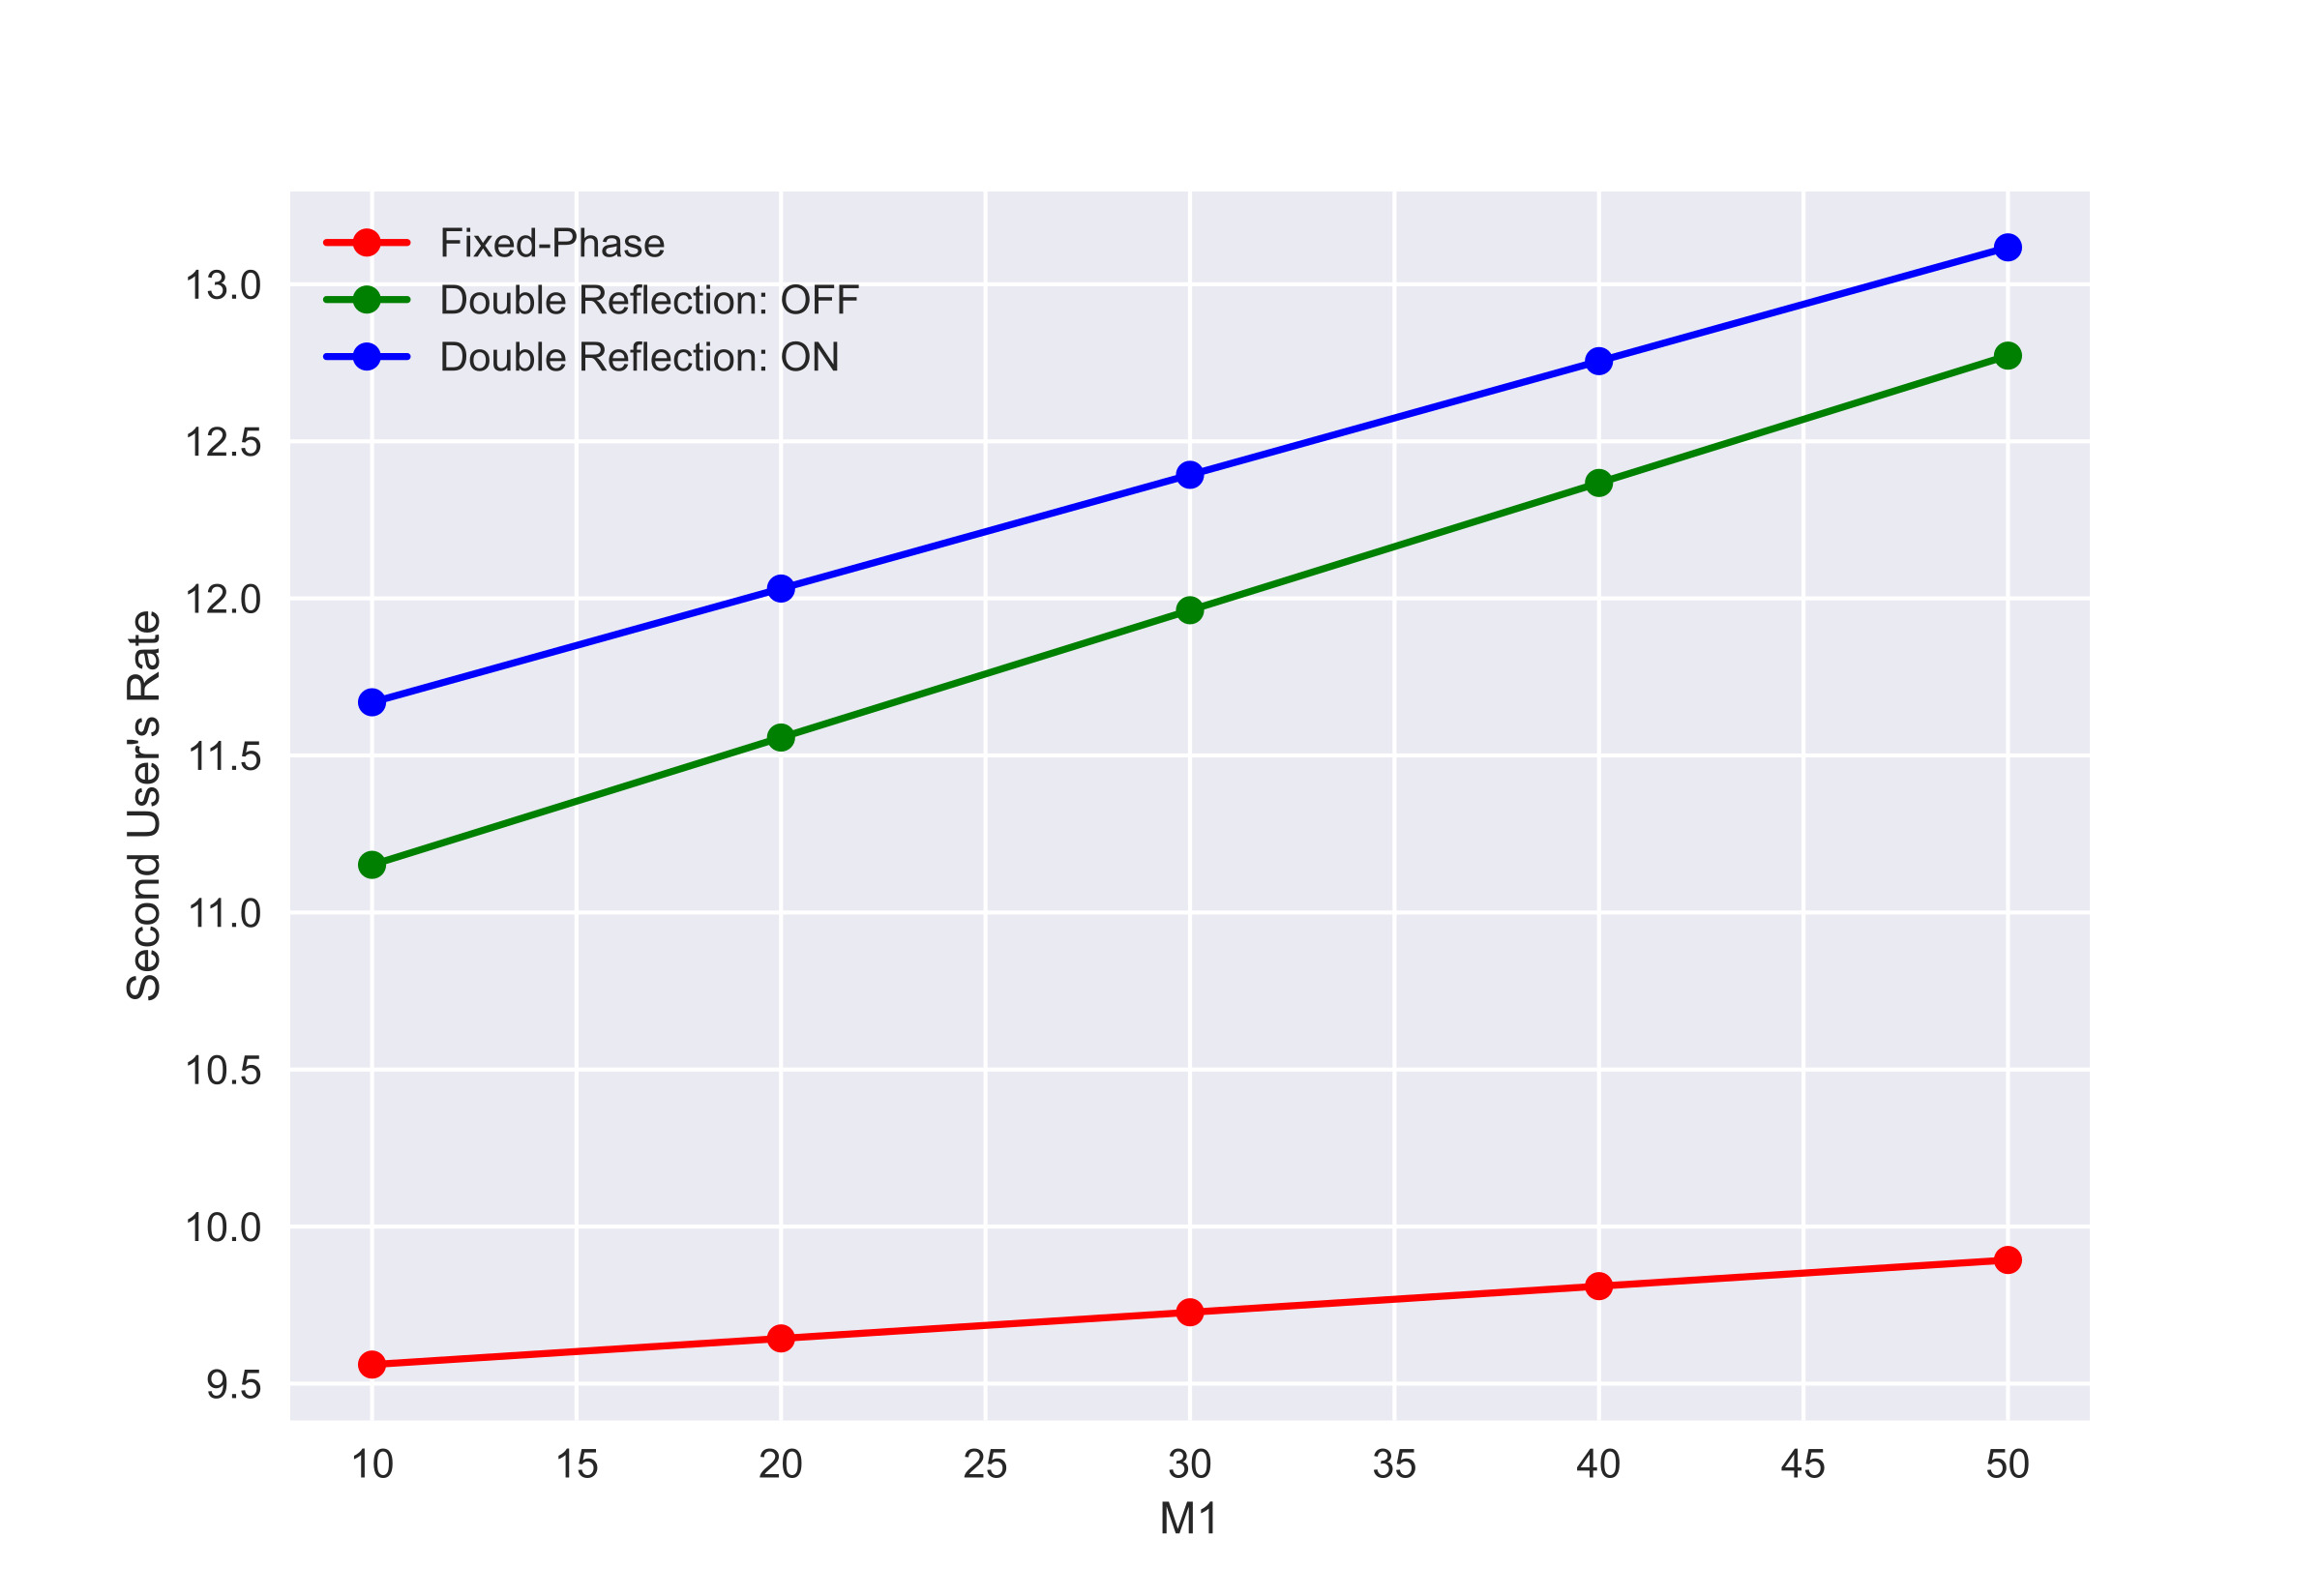
\includegraphics[scale=0.1]{No Blockage Second User's Rate}
		\captionsetup{width=0.8\linewidth}
		\caption[
		نرخ کاربر دوم در شرایط بدون مانع
		]{
		نرخ کاربر دوم در شرایط بدون مانع
		}
%		\label{fig:Picture-2_07}
	\end{minipage}
\end{figure}

\begin{figure}[!h]
	\centering
	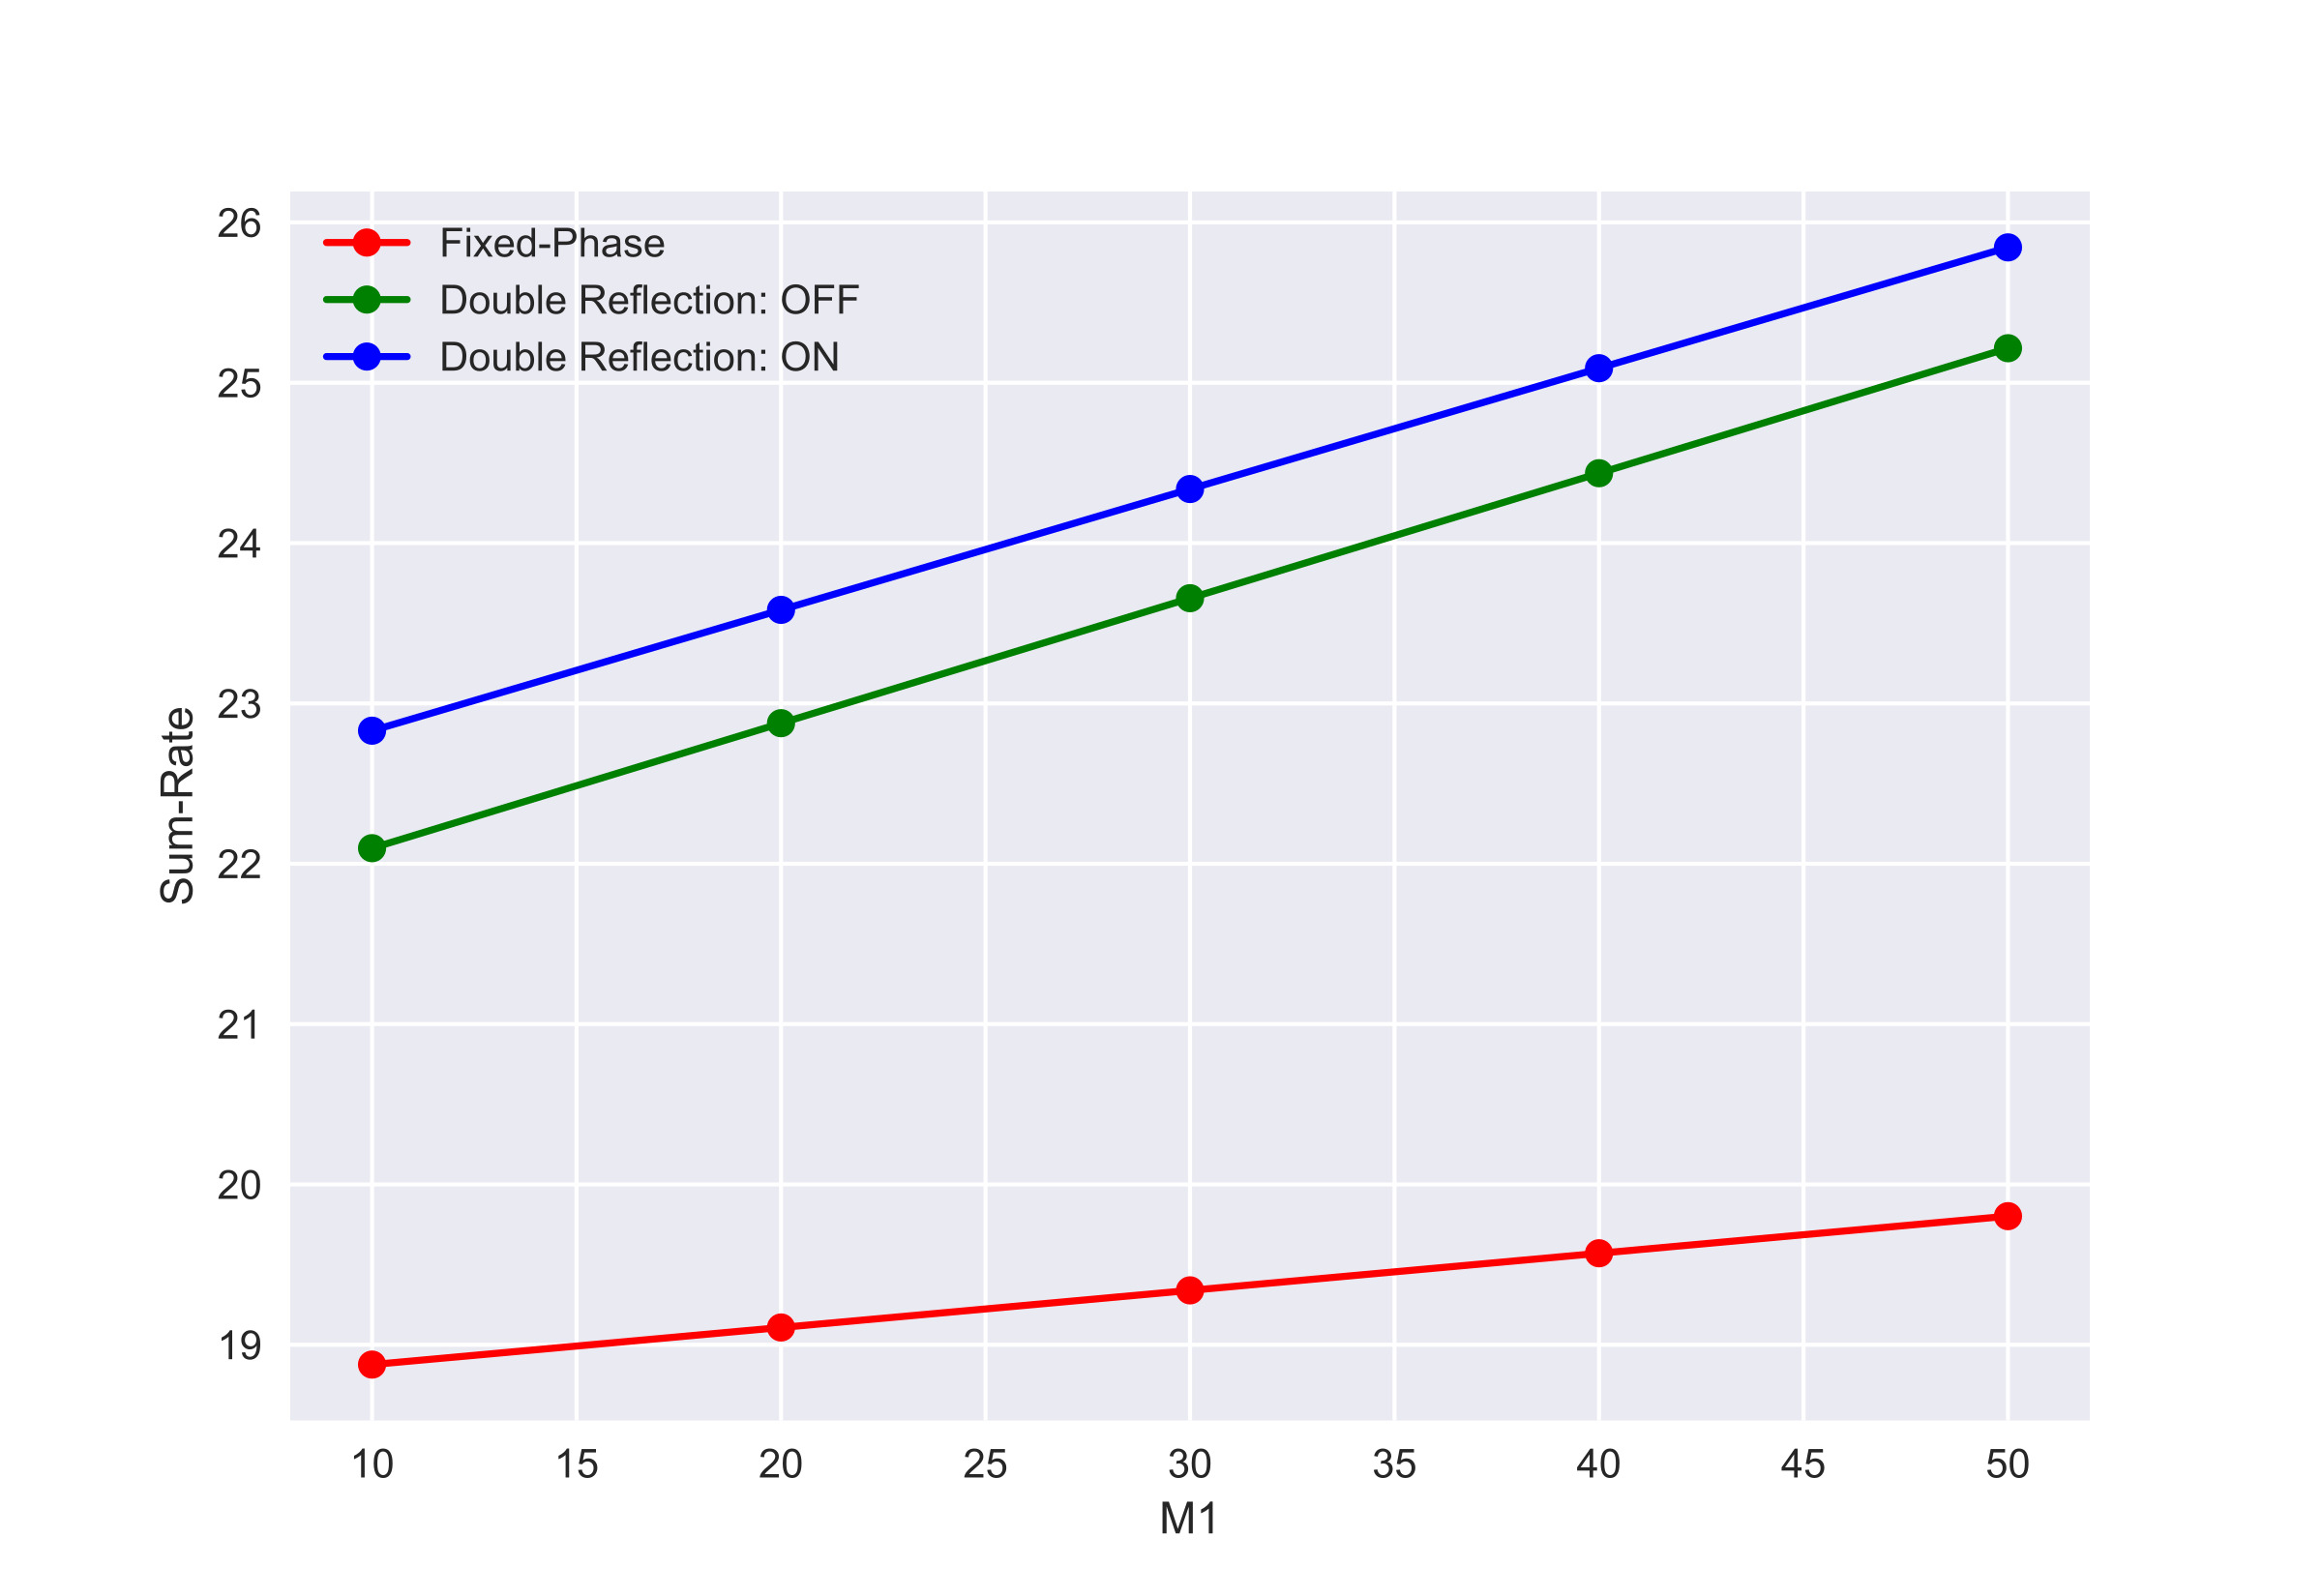
\includegraphics[scale=0.19]{No Blockage Sum-Rate}
	\caption[مجموع نرخ دو کاربر در شرایط بدون مانع]{
		مجموع نرخ دو کاربر در شرایط بدون مانع
	}
	%	\label{fig:fig-2_0}
\end{figure}

تحلیل: همانطور که مشاهده میشود در حالتی که سیگنال بازتابی بین سطوح در نظر گرفته شده‌است هر دو کاربر بهبودی را در سیگنال‌های دریافتی مشاهده میکنند اما نکته قابل توجه اینست که با در نظر گرفتن سیگنال بین سطوح باعث ایجاد پیچیدگی در بهینه‌سازی میشویم و زمان اجرا کندتر میشود و این موضوع میتواند سیستم را از حالت \lr{real time} خارج سازد پس باید هر شخص متناسب با سناریو خود بررسی کند که آیا این مقدار بهبود به اندازه پیچیدگی ایجاد شده ارزش دارد یا خیر؟
%%%%%%%%%%%%%%%%%%%%%%%%%%%%%%%%%%%%%%%%%%%
\newpage
\subsection{نتایج و تحلیل بهینه‌سازی با مانع}
طبق شرایط بالا و در حالت با مانع، شبیه‌سازی را اجرا کرده و نمودارهای زیر برای نرخ کاربر 1، کاربر 2 و مجموع نرخ هر دو کاربر رسم‌ شده ‌است:

\begin{figure}[!h]
	\begin{minipage}{0.5\textwidth}
		\centering
		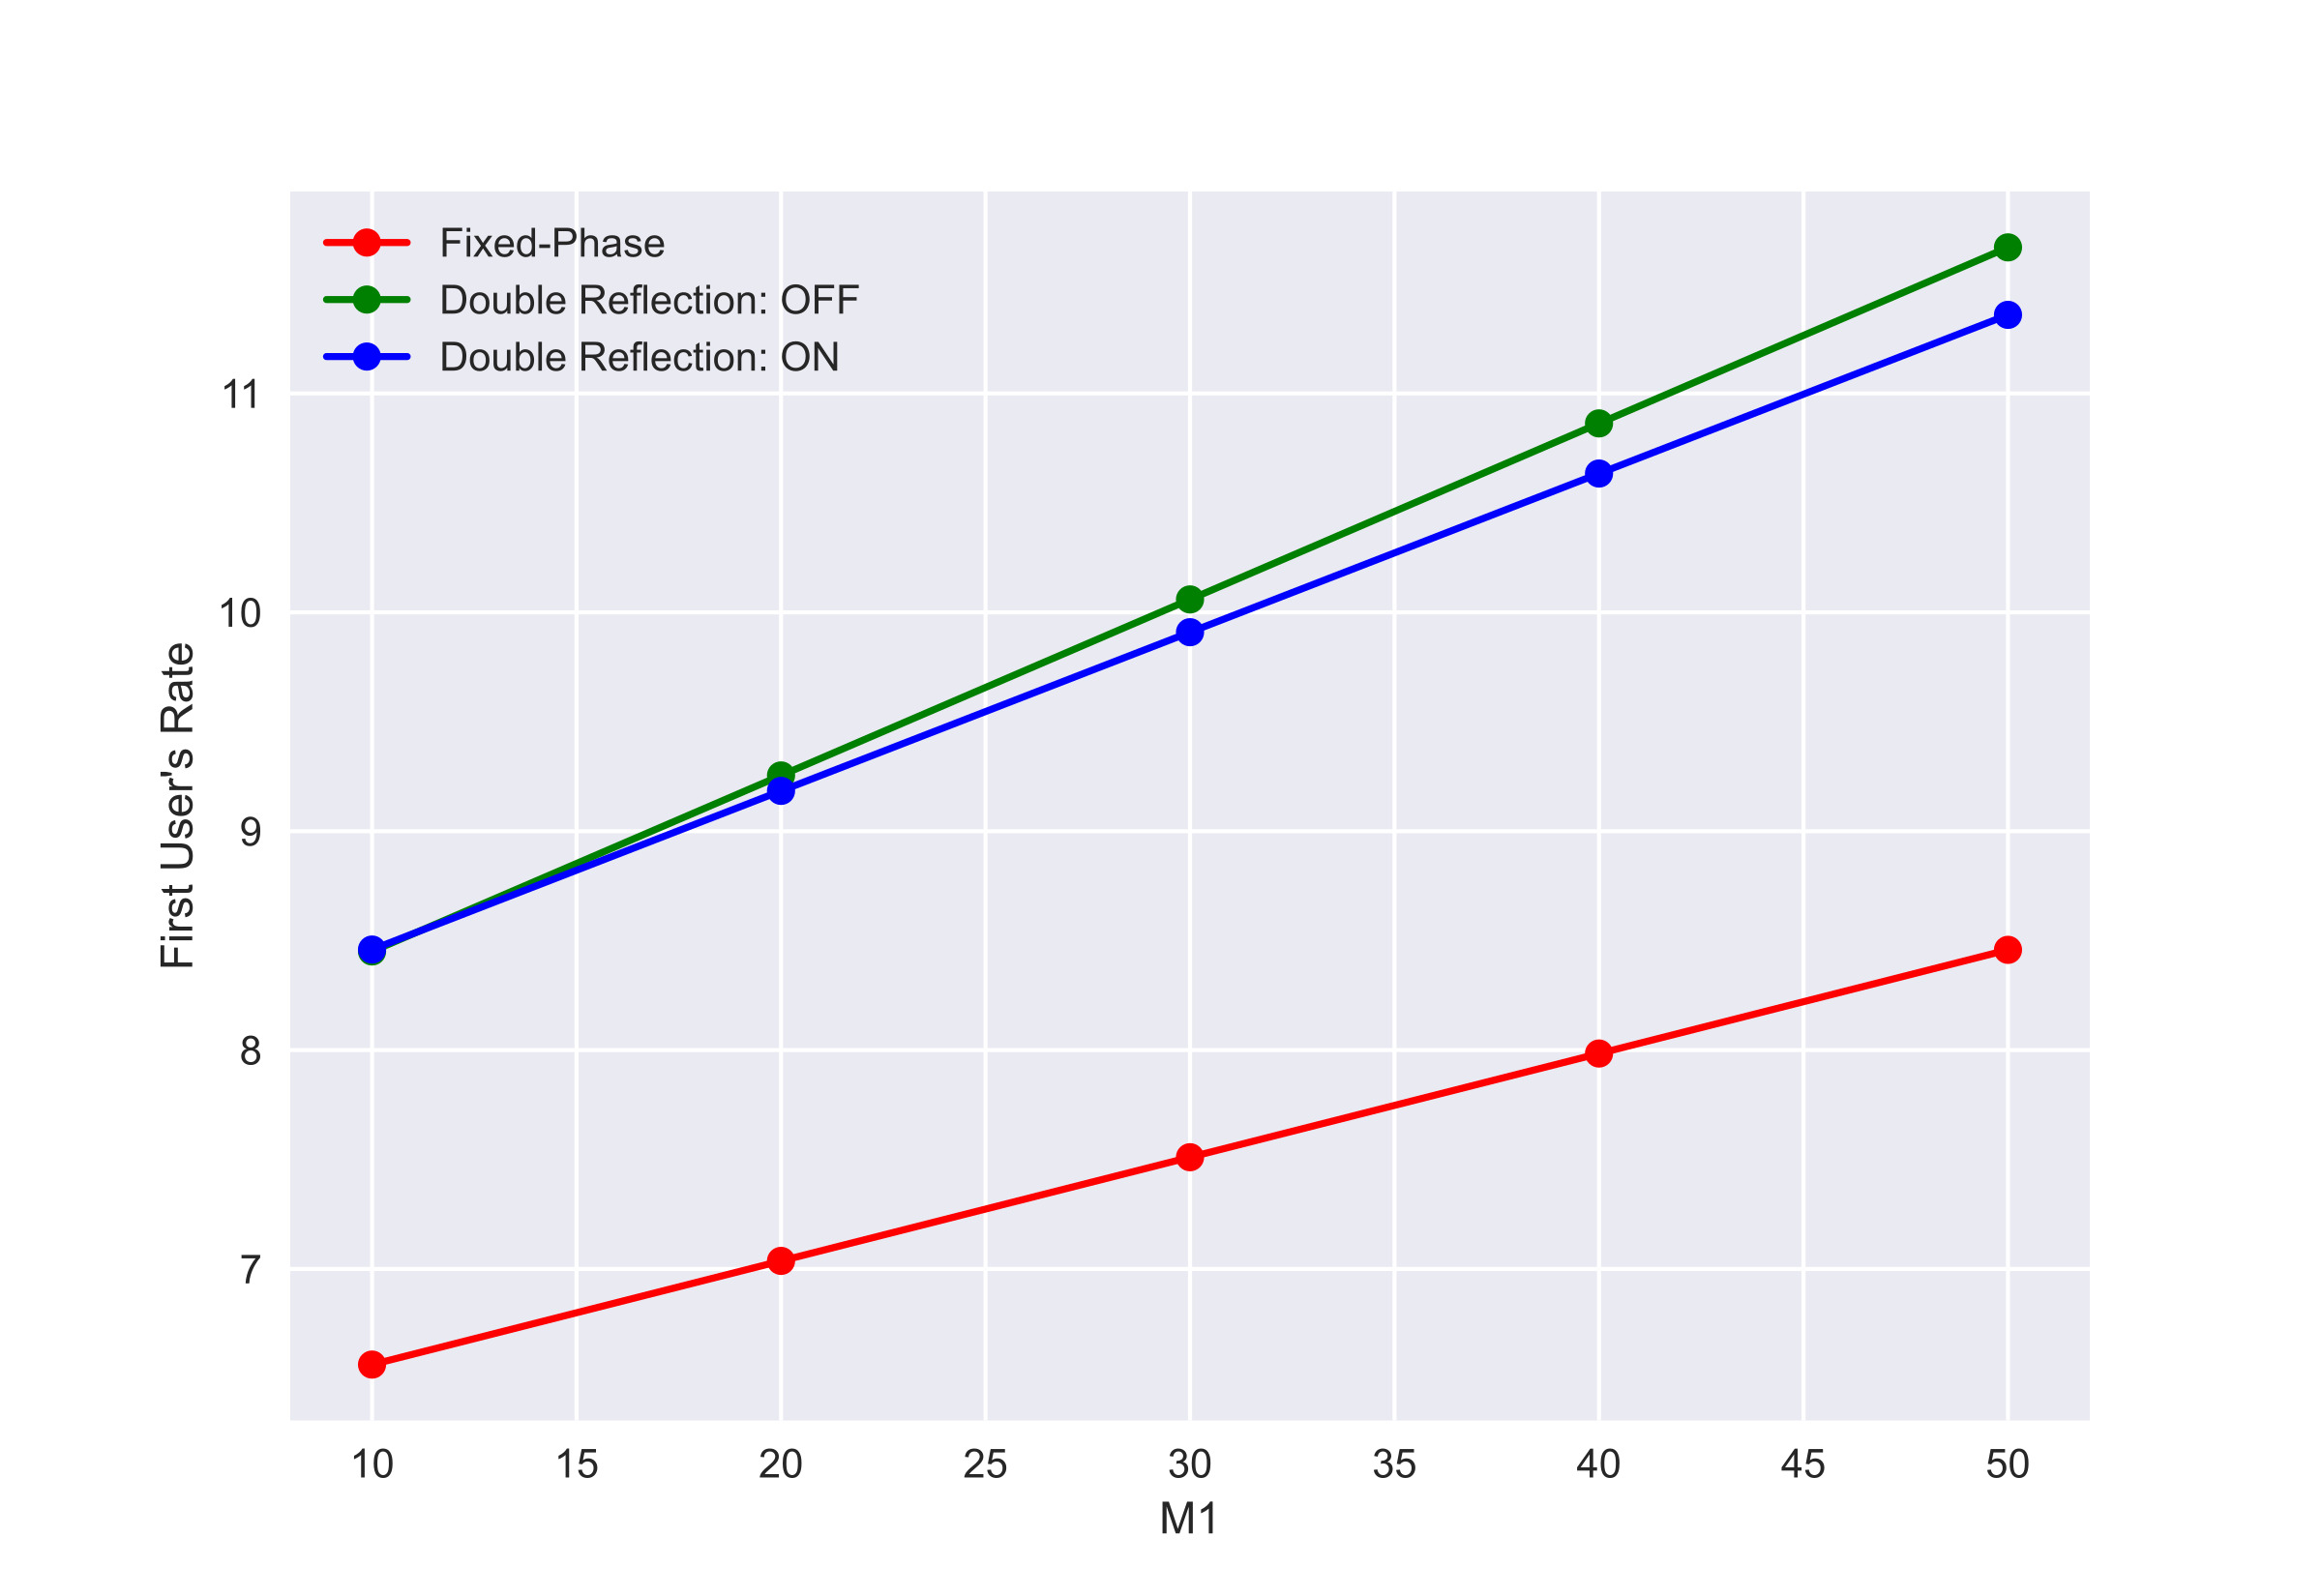
\includegraphics[scale=0.1]{With Blockage First User's Rate}
		\captionsetup{width=0.8\linewidth}
		\caption[
		نرخ کاربر اول در شرایط با مانع
		]{
		نرخ کاربر اول در شرایط با مانع
		}
%		\label{fig:Picture-2_006}
	\end{minipage}
	\hfill
	\begin{minipage}{0.5\textwidth}
		\centering
		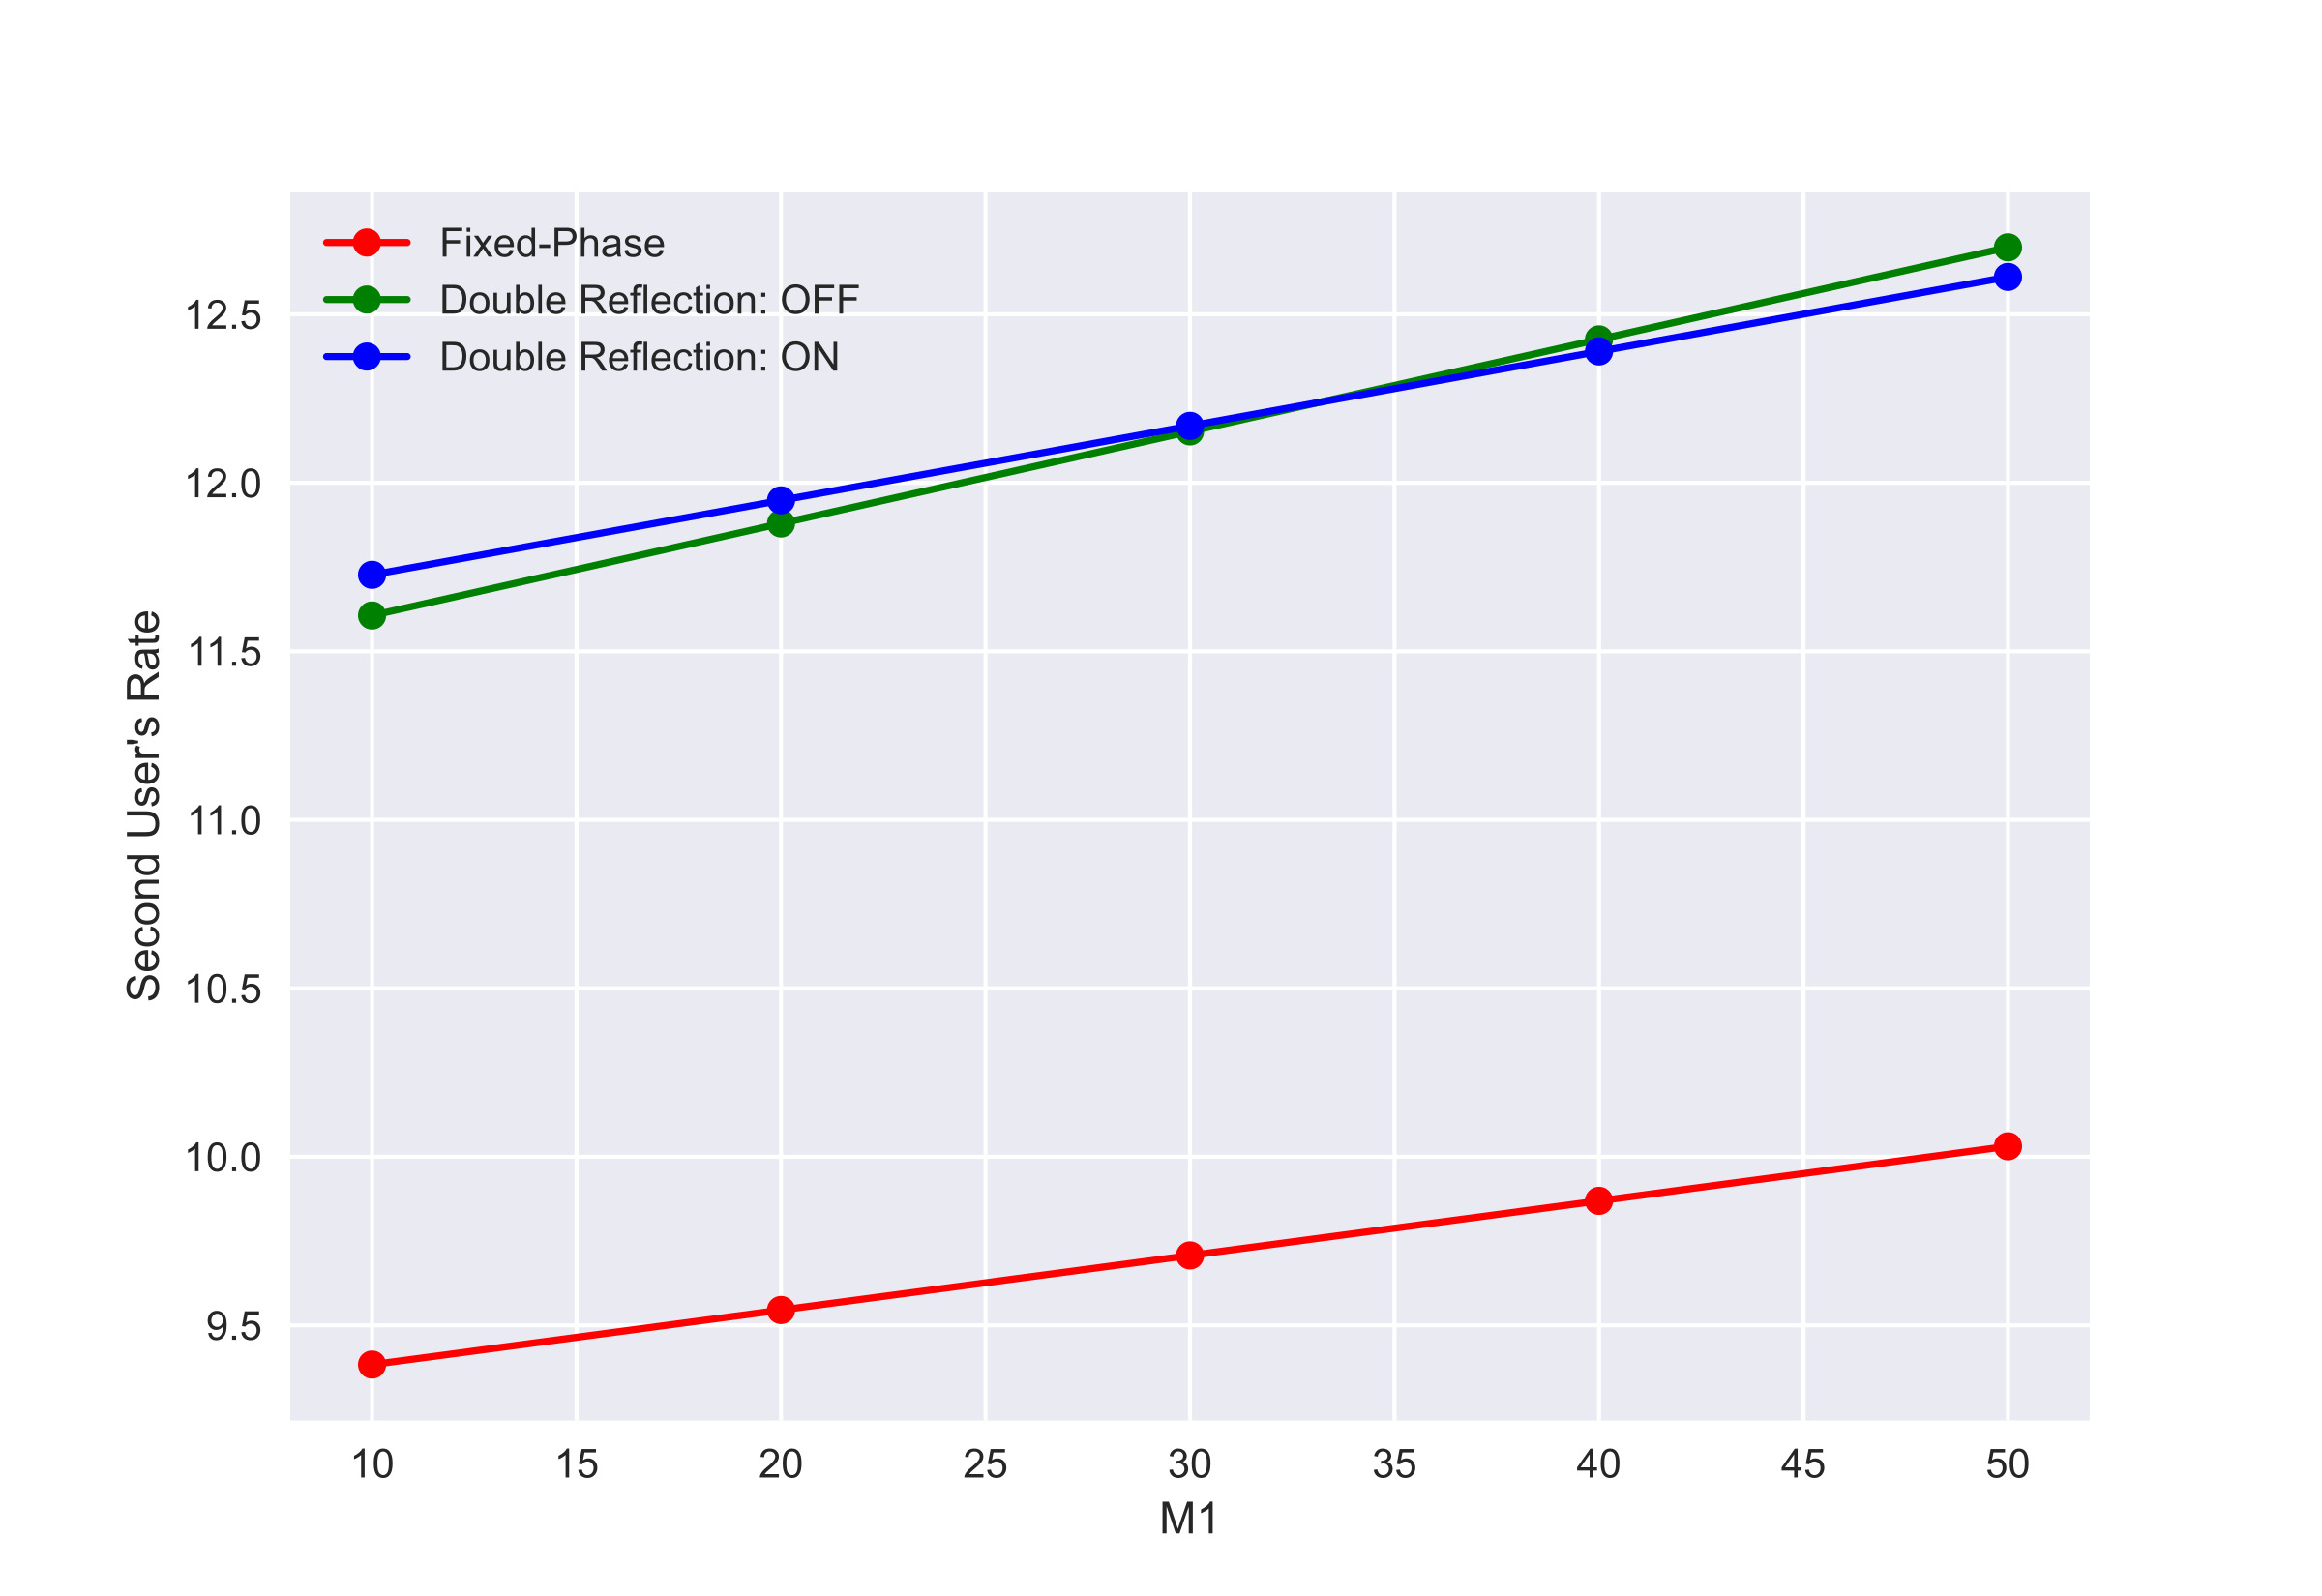
\includegraphics[scale=0.1]{With Blockage Second User's Rate}
		\captionsetup{width=0.8\linewidth}
		\caption[
		نرخ کاربر دوم در شرایط با مانع
		]{
			نرخ کاربر دوم در شرایط با مانع
		}
%		\label{fig:Picture-2_007}
	\end{minipage}
\end{figure}

\begin{figure}[!h]
	\centering
	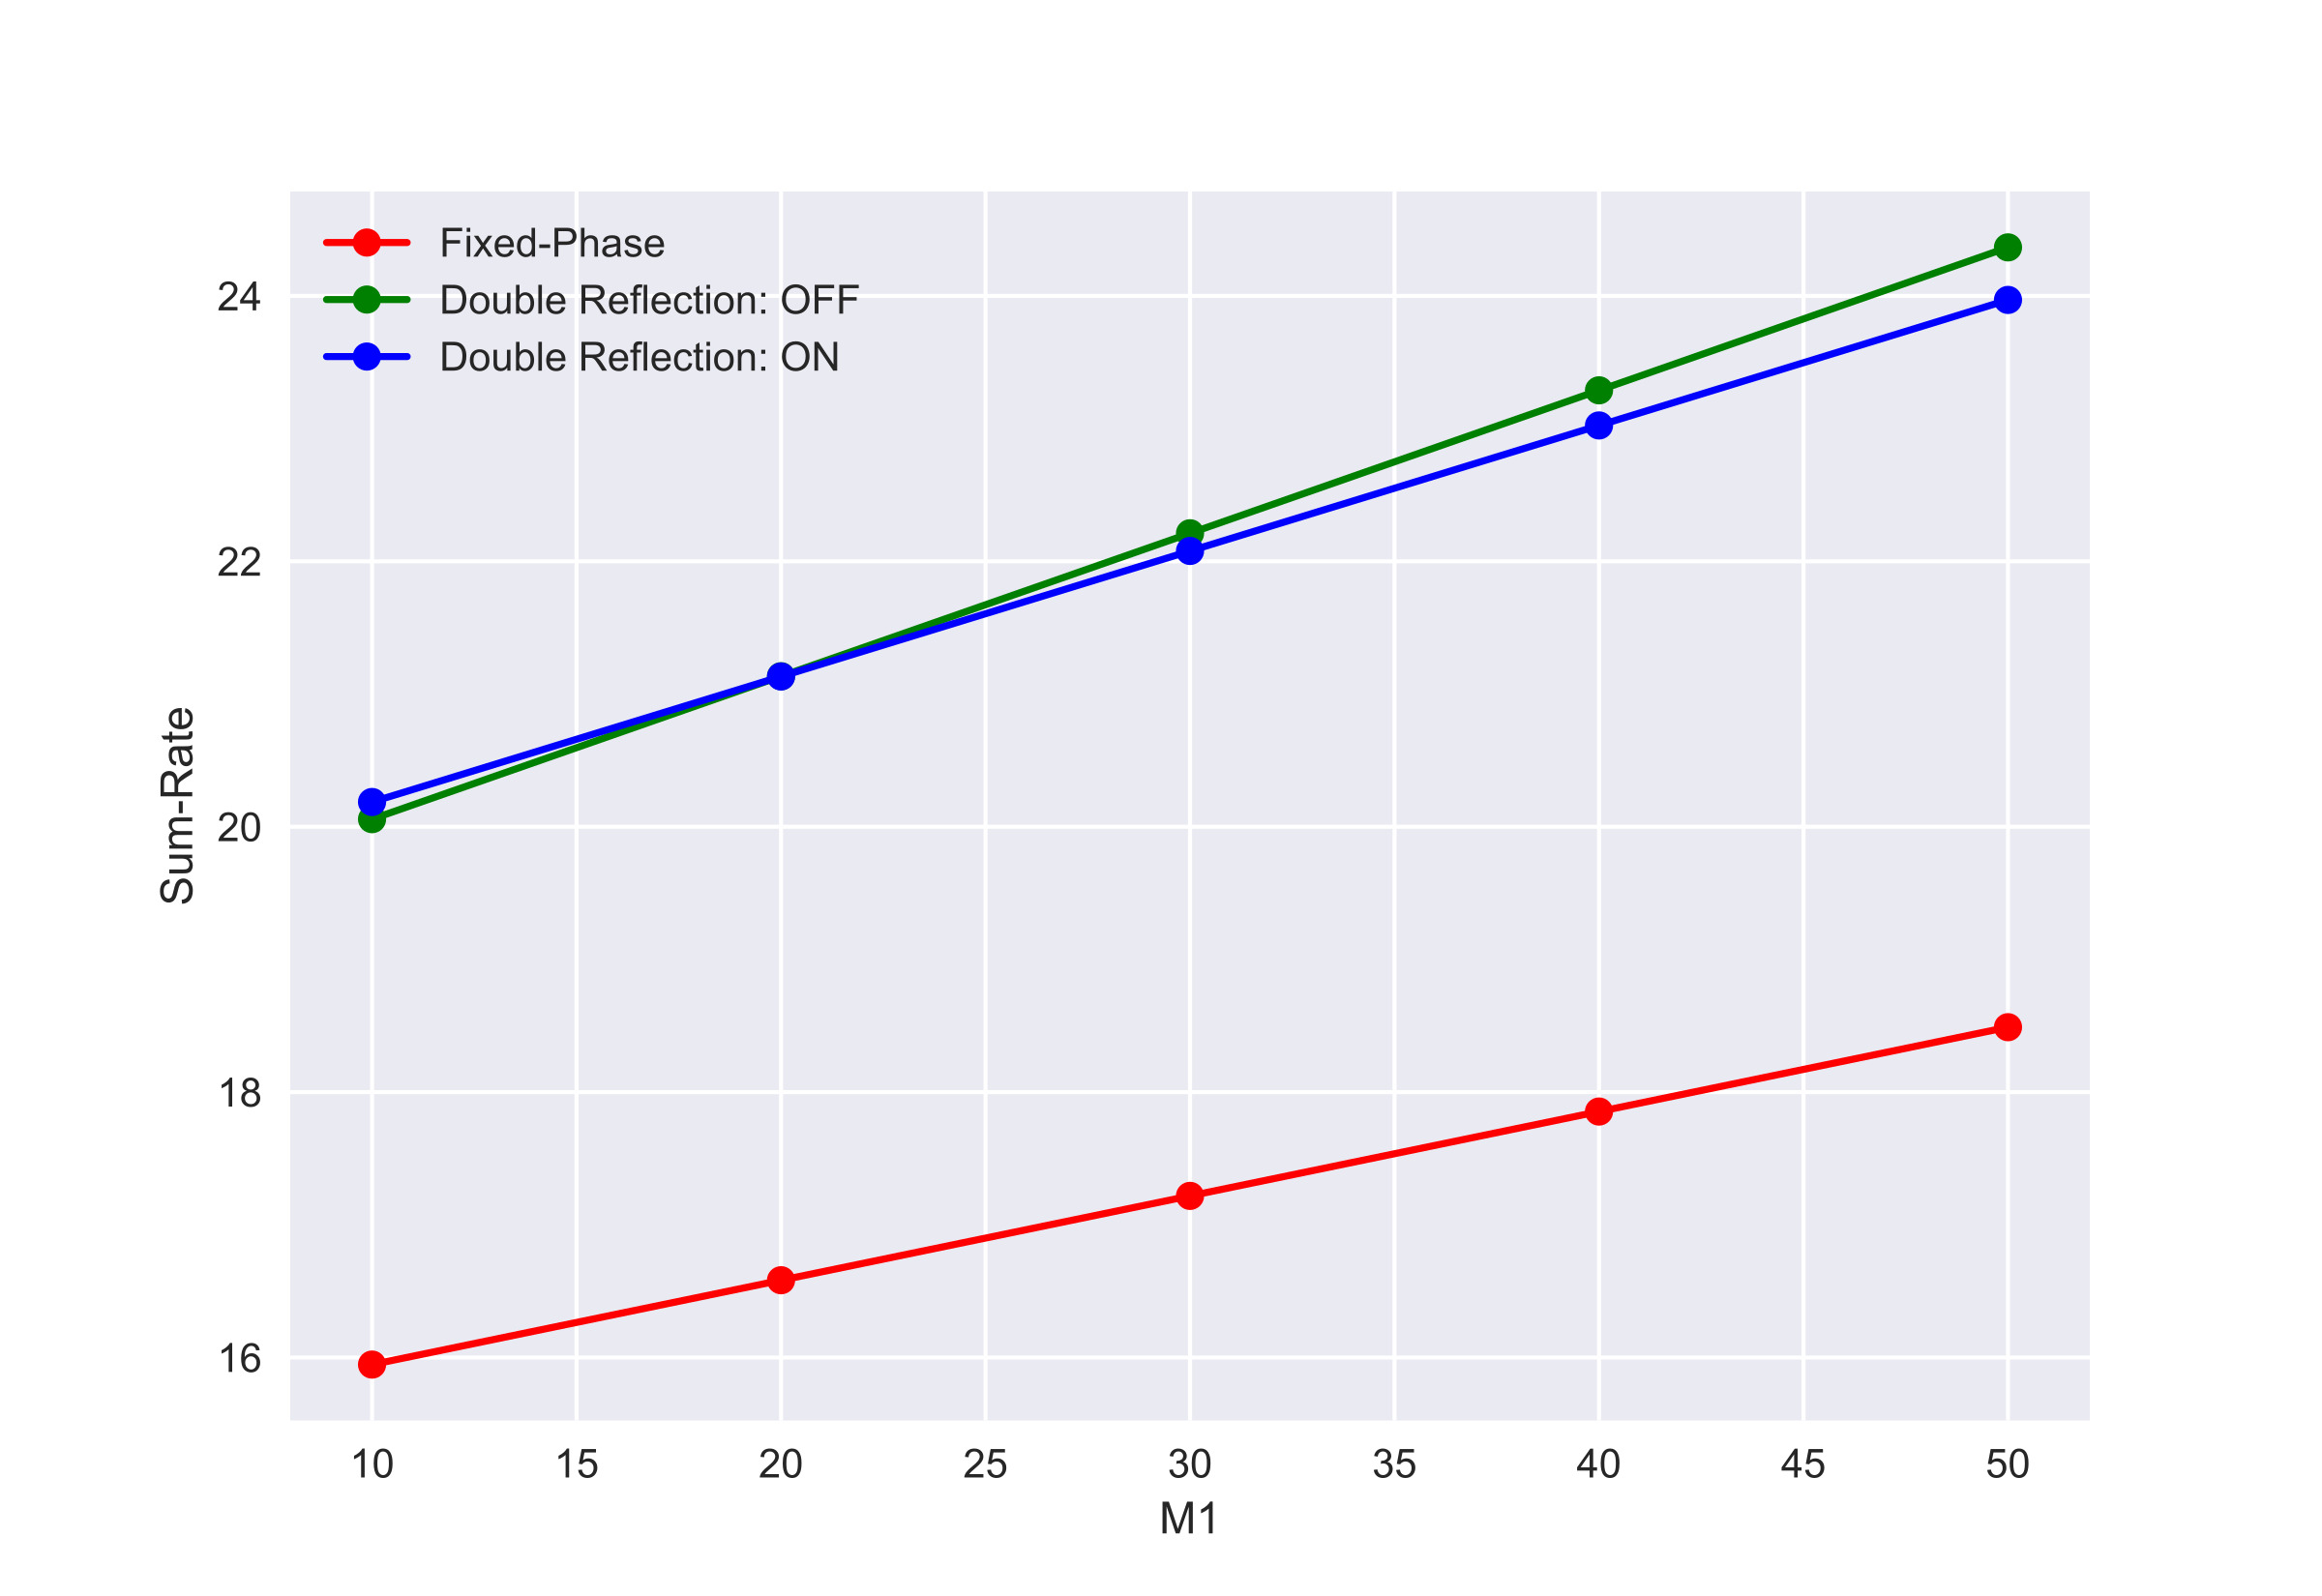
\includegraphics[scale=0.19]{With Blockage Sum-Rate}
	\caption[
	مجموع نرخ دو کاربر در شرایط با مانع
	]{
		مجموع نرخ دو کاربر در شرایط با مانع
	}
	%	\label{fig:fig-2_0}
\end{figure}

تحلیل: همانطور که مشاهده میشود در حالتی که سیگنال بازتابی بین سطوح در نظر گرفته شده‌است، هیچ‌یک از کاربرها بهبود خاصی را مشاهده نمیکنند و فقط با ایجاد پیچیدگی زمانی در مسئله، باعث کاهش سرعت همگرایی آن شده‌ایم. پس در این سناریو و سناریوهای مشابه استفاده از سیگنال بین سطوح توصیه نمیشود زیرا میتواند بدون هیچ بهبودی، باعث افزایش محاسبات و در نتیجه کاهش سرعت همگرایی شود.

\newpage
%%%%%%%%%%%%%%%%%%%%%%%%%%%%%%%%%%%%%%%%%%%
\section{پیشنهادات}

در این بخش به بررسی سه پیشنهاد(کارهای آینده) میپردازیم که میتواند توجه زیادی را به خود جلب کرده و مشکلات زیادی را حل کند:

\subsection{بازتاب مرتبه 3}

همانطور که دراین ستاریو بررسی شد، بازتاب بین سطوح هوشمند فقط تا بازتاب مرتبه 1 لحاظ شده است و در بخش نتایج مشاهده شد که این بازتاب، تاثیر چندانی بر روی بهینه شدن خروجی به نسبت پیچیدگی که به مسئله اضافه میکند، ندارد اما گاهی ناچار هستیم که این بازتاب را لحاظ کنیم. مثلا در هنگامی که دید مستقیم به فرستنده و یکی از دو سطوح هوشمند وجود ندارد، ناچار به لحاظ این بازتاب هستیم. 

اکنون یکی از مسائلی که مطرح میشود، این است که اگر 3 سطح هوشمند استفاده کنیم و دید مستقیم به دو سطح نداشته باشیم، آیا از نظر  نرخ دریافتی کاربر، بهینه است که از سیگنال بازتابی مرتبه 2 استفاده کنیم تا اطلاعات را به کاربر برسانیم؟

این یکی از سوالاتی است که میتواند در آینده و به کمک سایر محققان جواب داده شود. 

\subsection{ساخت فریم‌ورک برای بهینه‌سازی سطوح هوشمند}
یکی از چالش‌های اصلی که در برنامه‌نویسی این پروژه برای بهینه‌سازی ضرایب فاز وجود داشت، نبود هیچ فریم‌ورک یا همان چارچوب برنامه‌نویسی خاصی برای حل این مسائل است. ابتدا مجبور بودیم به دنبال الگوریتم بهینه بگردیم و سپس این الگوریتم را پیاده‌سازی نماییم و این امکان وجود داشت که الگوریتم مورد نظر در بیشینه‌های محلی غیر بهینه گیر کرده و نتواند به جواب قابل‌قبولی برسد. یا حتی ممکن بود این الگوریتم همگرا نشود که محقق در این صورت به ناچار مجبور است به سراغ سایر الگوریتم‌ها رفته که این کار اصلا از نظر زمان و انرژی، بهینه نیست.

اکنون میتوان به عنوان یکی از کارهای آینده، فریم‌ورکی طراحی کرد که کاربر، سناریو خود را به آن داده و این فریم‌ورک، انواع روش‌های مرسوم بهینه‌سازی در این حوزه را امتحان کرده و بهینه‌ترین جواب را انتخاب و به ما نمایش دهد.

البته که این مورد نیاز به صرف زمان و انرژی زیادی دارد که صرفا در قالب پروژه‌ای صنعتی و با وجود سرمایه‌گذار قابل انجام است.

\subsection{پیدا کردن طول گام بهینه}
یکی از مسائل مهم در سرعت همگرایی الگوریتم گرادیان نزولی، طول گامی است که انتخاب میکنیم. سال‌هاست که تحقیقاتی بر روی پیدا کردن روش های تطبیق‌پذیر برای یافتن طول گام بهینه انجام میشود. میتوان این الگوریتم‌ها را در این پروژه پیاده‌سازی کرد و نتایج بهتر و سریع‌تری گرفت. 
%%%%%%%%%%%%%%%%%%%%%%%%%%%%%%%%%%%%%%%%%%%
\newpage
‌

%--------------------------------------------------------------------------appendix( مراجع و پیوست ها)
\chapterfont{\vspace*{-2em}\centering\LARGE}%

\appendix
\bibliographystyle{unsrt-fa}
\bibliography{references}
\chapter*{‌پیوست}
\markboth{پیوست}{}
\addcontentsline{toc}{chapter}{پیوست}
موضوعات مرتبط با متن گزارش پایان نامه كه در يكی از گروه‌های زير قرار می‌گيرد، در بخش پيوست‌ها آورده شوند:
\begin{enumerate}
\item  اثبات های رياضی يا عمليات رياضی طولانی‌.‌
\item داده و اطلاعات نمونه (های) مورد مطالعه (\lr{Case Study}) چنانچه طولانی باشد‌.‌
\item نتايج كارهای ديگران چنانچه نياز به تفصيل باشد‌.‌
\item مجموعه تعاريف متغيرها و پارامترها، چنانچه طولانی بوده و در متن به انجام نرسيده باشد‌.‌
\end{enumerate}
% براي شماره‌گذاري روابط، جداول و اشكال موجود در پيوست‌ از ساختار متفاوتي نسبت به متن اصلي استفاده مي‌شود كه در زير به‌عنوان نمونه نمايش داده شده‌است. 
% \begin{equation}
%F=ma
%\end{equation}
\section*{کد میپل }
\begin{latin}
\begin{verbatim}

with(DifferentialGeometry):
with(Tensor):
DGsetup([x, y, z], M)
																	frame name: M
a := evalDG(D_x)
																	D_x
b := evalDG(-2 y z D_x+2 x D_y/z^3-D_z/z^2)


\end{verbatim}
\end{latin}
%--------------------------------------------------------------------------dictionary(واژه نامه ها)
%اگر مایل به داشتن صفحه واژه‌نامه نیستید، خط زیر را غیر فعال کنید.
\parindent=0pt
%
\chapter*{واژه‌نامه‌ی فارسی به انگلیسی}
\pagestyle{style9}

\addcontentsline{toc}{chapter}{واژه‌نامه‌ی فارسی به انگلیسی}
%%%%%%
\begin{multicols*}{2}

{\bf آ}
\vspace*{3mm}


\farsiTOenglish{ایستگاه زمینی}{BTS}
\farsiTOenglish{انتقال انرژی}{Energy Harvesting}


\vspace*{3mm}
{\bf ب}
\vspace*{3mm}

\farsiTOenglish{برنامه‌ریزی درجه دوم}{Quadratic Programming}
\farsiTOenglish{برنامه‌ریزی خطی}{Linear Programming}
\farsiTOenglish{بهینه‌سازی کلاسیک}{Classic Optimization}
\farsiTOenglish{بهینه‌سازی محدب}{Convex Optimization}
\farsiTOenglish{برنامه‌ریزی چند کسیری}{Multi-Fractional Programming}


%\vspace*{3mm}
%{\bf پ}
%%\vspace*{3mm}

%\farsiTOenglish{پایا}{Invariant}



\vspace*{3mm}
{\bf ت}
%%\vspace*{3mm}

\farsiTOenglish{ تک ورودی تک خروجی }{SISO}
\farsiTOenglish{ تک ورودی چند خروجی }{SIMO}
\farsiTOenglish{ توان }{Power}

%\vspace*{3mm}
%{\bf ث}
%%\vspace*{3mm}

%\farsiTOenglish{ثابت‌ساز}{Stabilizer}

\vspace*{3mm}
{\bf ج}
%%\vspace*{3mm}

\farsiTOenglish{جستجوی دوبخشی}{Bisection Search}



\vspace*{3mm}
{\bf چ}
%%\vspace*{3mm}


\farsiTOenglish{چند ورودی تک خروجی }{MISO}
\farsiTOenglish{چند ورودی چند خروجی }{MIMO}

%\vspace*{3mm}
%{\bf ح}
%%\vspace*{3mm}

%\farsiTOenglish{حاصل‌ضرب دکارتی}{Cartesian product}


%\vspace*{3mm}
%{\bf خ}
%%\vspace*{3mm}

%\farsiTOenglish{خودریختی}{Automorphism}

\vspace*{3mm}
{\bf د}
%%\vspace*{3mm}

\farsiTOenglish{داده}{Data}
\farsiTOenglish{دوگانگی لاگرانژی}{Lagrangian Duality}

%\vspace*{3mm}
%{\bf ر}
%%\vspace*{3mm}


%\farsiTOenglish{ریزپردازنده}{microprocessor}


%\vspace*{3mm}
%{\bf ز}
%%\vspace*{3mm}


%\farsiTOenglish{زیرمدول}{Submodule}


%\vspace*{3mm}
%{\bf س}
%%\vspace*{3mm}

\farsiTOenglish{سطح بازتاب دهنده هوشمند}{Intelligent Reflective Surface}


%\vspace*{3mm}
%{\bf ص}
%%\vspace*{3mm}

%\farsiTOenglish{صادقانه}{Faithful}

%\vspace*{3mm}
%{\bf ض}
%%\vspace*{3mm}

%\farsiTOenglish{ضرب داخلی}{Inner product}

%\vspace*{3mm}
%{\bf ط}
%%\vspace*{3mm}


%\farsiTOenglish{طوقه}{Loop}


%\vspace*{3mm}
%{\bf ظ}
%%\vspace*{3mm}


%\farsiTOenglish{ظرفیت}{Valency}
 
\vspace*{3mm}
{\bf ع}
%%\vspace*{3mm}


\farsiTOenglish{عظیم}{Massive}


\vspace*{3mm}
{\bf غ}
%%\vspace*{3mm}


\farsiTOenglish{غیر فعال}{Passive}


%\vspace*{3mm}
%{\bf ف}
%%\vspace*{3mm}

%\farsiTOenglish{فضای برداری}{Vector space}



\vspace*{3mm}
{\bf ک}
%%\vspace*{3mm}

\farsiTOenglish{کدگذاری}{Encode}
\farsiTOenglish{کدگشایی}{Decode}


%\vspace*{3mm}
%{\bf گ}
%%\vspace*{3mm}


%\farsiTOenglish{گراف}{Graph}



\vspace*{3mm}
{\bf م}
%%\vspace*{3mm}

\farsiTOenglish{مدولاسیون}{Modulation}
\farsiTOenglish{مخابرات سلولی}{Cellular Communication}
\farsiTOenglish{مختصات نزولی}{Coordinate Descent}
\farsiTOenglish{مشتق نزولی}{Gradient Descent}


%\vspace*{3mm}
%{\bf ن}
%%\vspace*{3mm}

%\farsiTOenglish{ناهمبند}{Disconnected}


%\vspace*{3mm}
%{\bf و}
%%\vspace*{3mm}

%\farsiTOenglish{وارون‌پذیر}{Invertible}


\vspace*{3mm}
{\bf ه}
%%\vspace*{3mm}

\farsiTOenglish{هوش مصنوعی}{Artificial Intelligence}



%\vspace*{3mm}
%{\bf ی}
%%\vspace*{3mm}

%\farsiTOenglish{یال}{Edge}




\end{multicols*}%
%%%%%%
\chapter*{ واژه‌نامه‌ی انگلیسی به فارسی}
\pagestyle{style9}
\lhead{\thepage}\rhead{واژه‌نامه‌ی انگلیسی به فارسی}
\addcontentsline{toc}{chapter}{واژه‌نامه‌ی انگلیسی به فارسی}

\LTRmulticolcolumns
\begin{multicols}{2}
{\hfill\bf  \lr{A}}
%%\vspace*{1.5mm}

\englishTOfarsi{Artificial Intelligence}{هوش مصنوعی}

\vspace*{3mm}
{\hfill\bf   \lr{B}}
%%\vspace*{1.5mm}

\englishTOfarsi{BTS}{ایستگاه زمینی}
\englishTOfarsi{Bisection Search}{جستجوی دوبخشی}

\vspace*{3mm}
{\hfill\bf   \lr{C}}
%%\vspace*{1.5mm}

\englishTOfarsi{Classic Optimization}{بهینه‌سازی کلاسیک}
\englishTOfarsi{Convex Optimization}{بهینه‌سازی محدب}
\englishTOfarsi{Cellular Communication}{مخابرات سلولی}
\englishTOfarsi{Coordinate Descent}{مختصات نزولی}



\vspace*{3mm}
{\hfill\bf   \lr{D}}
%%\vspace*{1.5mm}

\englishTOfarsi{Data}{داده}
\englishTOfarsi{Decode}{کدگشایی}


\vspace*{3mm}
{\hfill\bf   \lr{E}}
%%\vspace*{1.5mm}

\englishTOfarsi{Energy Harvesting}{انتقال انرژی}
\englishTOfarsi{Encode}{کدگذاری}


%\vspace*{3mm}
%{\hfill\bf   \lr{F}}
%%\vspace*{1.5mm}

%\englishTOfarsi{Function}{تابع}

\vspace*{3mm}
{\hfill\bf   \lr{G}}
%%\vspace*{1.5mm}

\englishTOfarsi{Gradient Descent}{مشتق نزولی}

%\vspace*{3mm}
%{\hfill\bf   \lr{H}}
%%\vspace*{1.5mm}

%\englishTOfarsi{Homomorphism}{همریختی}

\vspace*{3mm}
{\hfill\bf   \lr{I}}
%%\vspace*{1.5mm}

\englishTOfarsi{Intelligent Reflective Surface}{سطح بازتاب دهنده هوشمند}

\vspace*{3mm}
{\hfill\bf   \lr{L}}
%%\vspace*{1.5mm}

\englishTOfarsi{Linear Programming}{برنامه‌ریزی خطی}
\englishTOfarsi{Lagrangian Duality}{دوگانگی لاگرانژی}


\vspace*{3mm}
{\hfill\bf   \lr{M}}
%%\vspace*{1.5mm}

\englishTOfarsi{Multi-Fractional Programming}{برنامه‌ریزی چند کسیری}
\englishTOfarsi{MISO}{چند ورودی تک خروجی }
\englishTOfarsi{MIMO}{چند ورودی چند خروجی }
\englishTOfarsi{Massive}{عظیم}
\englishTOfarsi{Modulation}{مدولاسیون}



%\vspace*{3mm}
%{\hfill\bf   \lr{N}}
%%\vspace*{1.5mm}

%\englishTOfarsi{Natural map}{نگاشت طبیعی}

%\vspace*{3mm}
%{\hfill\bf   \lr{O}}
%%\vspace*{1.5mm}

%\englishTOfarsi{One to One}{یک به یک}

\vspace*{3mm}
{\hfill\bf   \lr{P}}
%%\vspace*{1.5mm}

\englishTOfarsi{Power}{ توان }
\englishTOfarsi{Passive}{غیر فعال}


\vspace*{3mm}
{\hfill\bf   \lr{Q}}
%%\vspace*{1.5mm}

\englishTOfarsi{Quadratic Programming}{برنامه‌ریزی درجه دوم}

% \vspace*{3mm}
%{\hfill\bf   \lr{R}}
%%\vspace*{1.5mm}

%\englishTOfarsi{Reducible}{تحویل پذیر}

\vspace*{3mm}
{\hfill\bf   \lr{S}}
%%\vspace*{1.5mm}

\englishTOfarsi{SISO}{ تک ورودی تک خروجی }
\englishTOfarsi{SIMO}{ تک ورودی چند خروجی }

% \vspace*{3mm}
%{\hfill\bf   \lr{T}}
%%\vspace*{1.5mm}

%\englishTOfarsi{Trivial character}{سرشت بدیهی}

%\vspace*{3mm}
%{\hfill\bf   \lr{U}}
%%\vspace*{1.5mm}

%\englishTOfarsi{Unique}{منحصربفرد}

%\vspace*{3mm}
%{\hfill\bf   \lr{V}}
%%\vspace*{1.5mm}

%\englishTOfarsi{Vector space}{فضای برداری}

\end{multicols}
%--------------------------------------------------------------------------index(نمایه)
%اگر مایل به داشتن صفحه نمایه نیستید، خط زیر را غیر فعال کنید.
\pagestyle{style7}
\printindex
\pagestyle{style7}
%کلمات کلیدی انگلیسی
\latinkeywords{IRS, Double Reflection, Sum-Rate, Coordinate Descent, Gradient Descent}
%چکیده انگلیسی

\en-abstract{
This research explores the potential application of Intelligent Reflecting Surfaces (IRS) in the context of future communication networks, specifically focusing on 6G.
The study aims to optimize the weighted-sum-rate objective function for a realistic scenario involving two users.
In this scenario, the collaboration of two IRS units is considered, with a second-order reflection occurring between them.
One of the users experiences an obstacle, highlighting the need for improved network performance.
To enhance the communication network’s performance, a joint optimization approach is employed, optimizing both the passive beamforming coefficients of the IRS and the active beamforming coefficients of the antenna.
This optimization is carried out using a coordinate descent algorithm consisting of a gradient descent inside it, which iteratively refines the beamforming coefficients to maximize the overall system performance. 
The research also includes an evaluation of the Signal-to Interference-plus-Noise Ratio (SINR) improvement in the presence of the second-order reflection between the two IRS units.
The optimization process comprises several key steps.
Firstly, the Lagrangian dual transformation is applied to eliminate the logarithmic function, simplifying the optimization problem.
This transformation facilitates a more efficient and tractable optimization process.
Additionally, fractional programming techniques are employed to convert fractional terms into linear functions, further streamlining the optimization process.
These optimization techniques enable the exploration of optimal beamforming strategies and pave the way for enhanced performance in future wireless communication systems.
}
%%%%%%%%%%%%%%%%%%%%% کدهای زیر را تغییر ندهید.

\newpage
\thispagestyle{empty}
\begin{latin}
\section*{\LARGE\centering Abstract}

\een-abstract

\vspace*{.5cm}
{\large\textbf{Key Words:}}\par
\vspace*{.5cm}
\elatinkeywords
\end{latin}
% در این فایل، عنوان پایان‌نامه، مشخصات خود و چکیده پایان‌نامه را به انگلیسی، وارد کنید.
%%%%%%%%%%%%%%%%%%%%%%%%%%%%%%%%%%%%
\baselineskip=.6cm
\begin{latin}

\latinfaculty{Department of ...}


\latintitle{Title of Thesis}


\firstlatinsupervisor{Dr. }

%\secondlatinsupervisor{Second Supervisor}

\firstlatinadvisor{Dr. }

%\secondlatinadvisor{Second Advisor}

\latinname{Name}

\latinsurname{Surname}

\latinthesisdate{Month \& Year}

\latinvtitle
\end{latin}

\end{document}